\subsection{Результаты моделирования}

Оценивалась работа 3х алгоритмов:
\begin{mintemize}
\item случайное перемещение
\item поиск ближайших неизведанных зон
\item равномерное распределение по карте
\end{mintemize}

Как критерий оценки использовалось состояние карты на момент
времени $T$ работы системы. В состояние карты входят:

\begin{mintemize}
\item соотношение количества известных секторов к общему
\item средняя разница между последней проверкой и текущим временем
    для известных секторов карты
\end{mintemize}

Для каждого алгоритма было произведено 3 эксперимента с разным
количеством юнитов: 16, 33, 50.

Графики строились в программе \verb|gnuplot|, информация для
построения генерировалась ПМО.

\newpage
\subsubsection{Случайное перемещение}

\begin{figure}[h!]
    \centering
    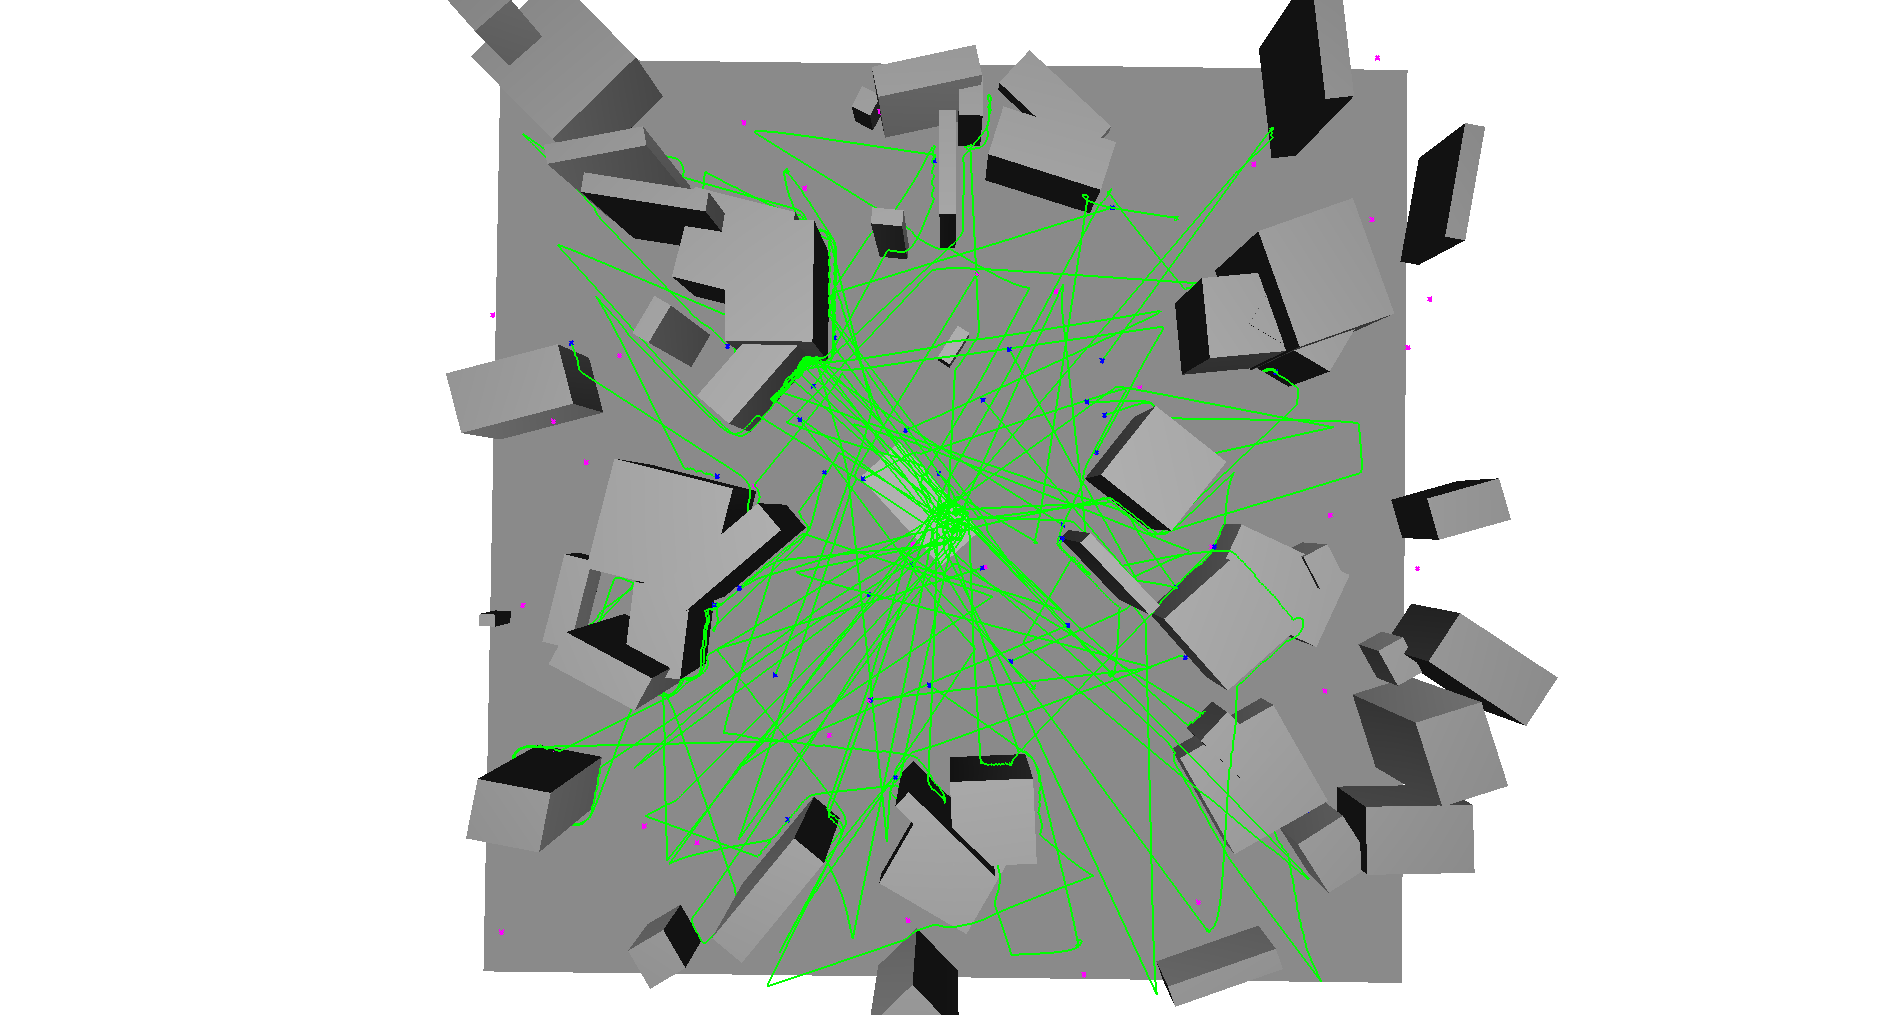
\includegraphics[width=\linewidth]{s50rm_view.png}
    \caption{Случайное перемещение, 50 юнитов, вид сверху, пути перемещения}
\end{figure}

\begin{figure}[h!]
    \centering
    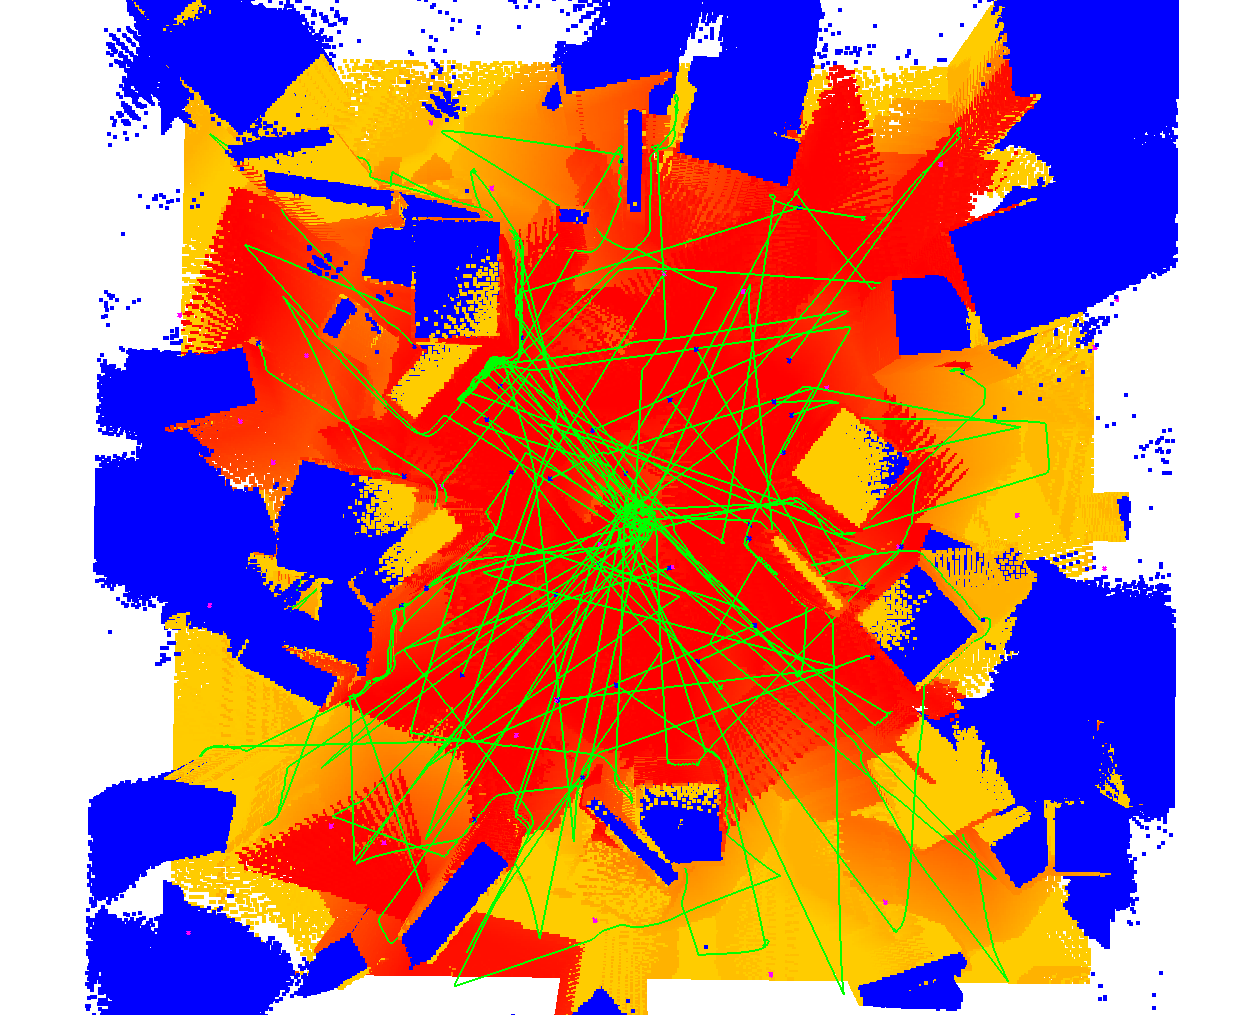
\includegraphics[width=\linewidth]{s50rm_map.png}
    \caption{Случайное перемещение, 50 юнитов, вид сверху, состояние карты}
\end{figure}

\begin{figure}[h!]
    \centering
    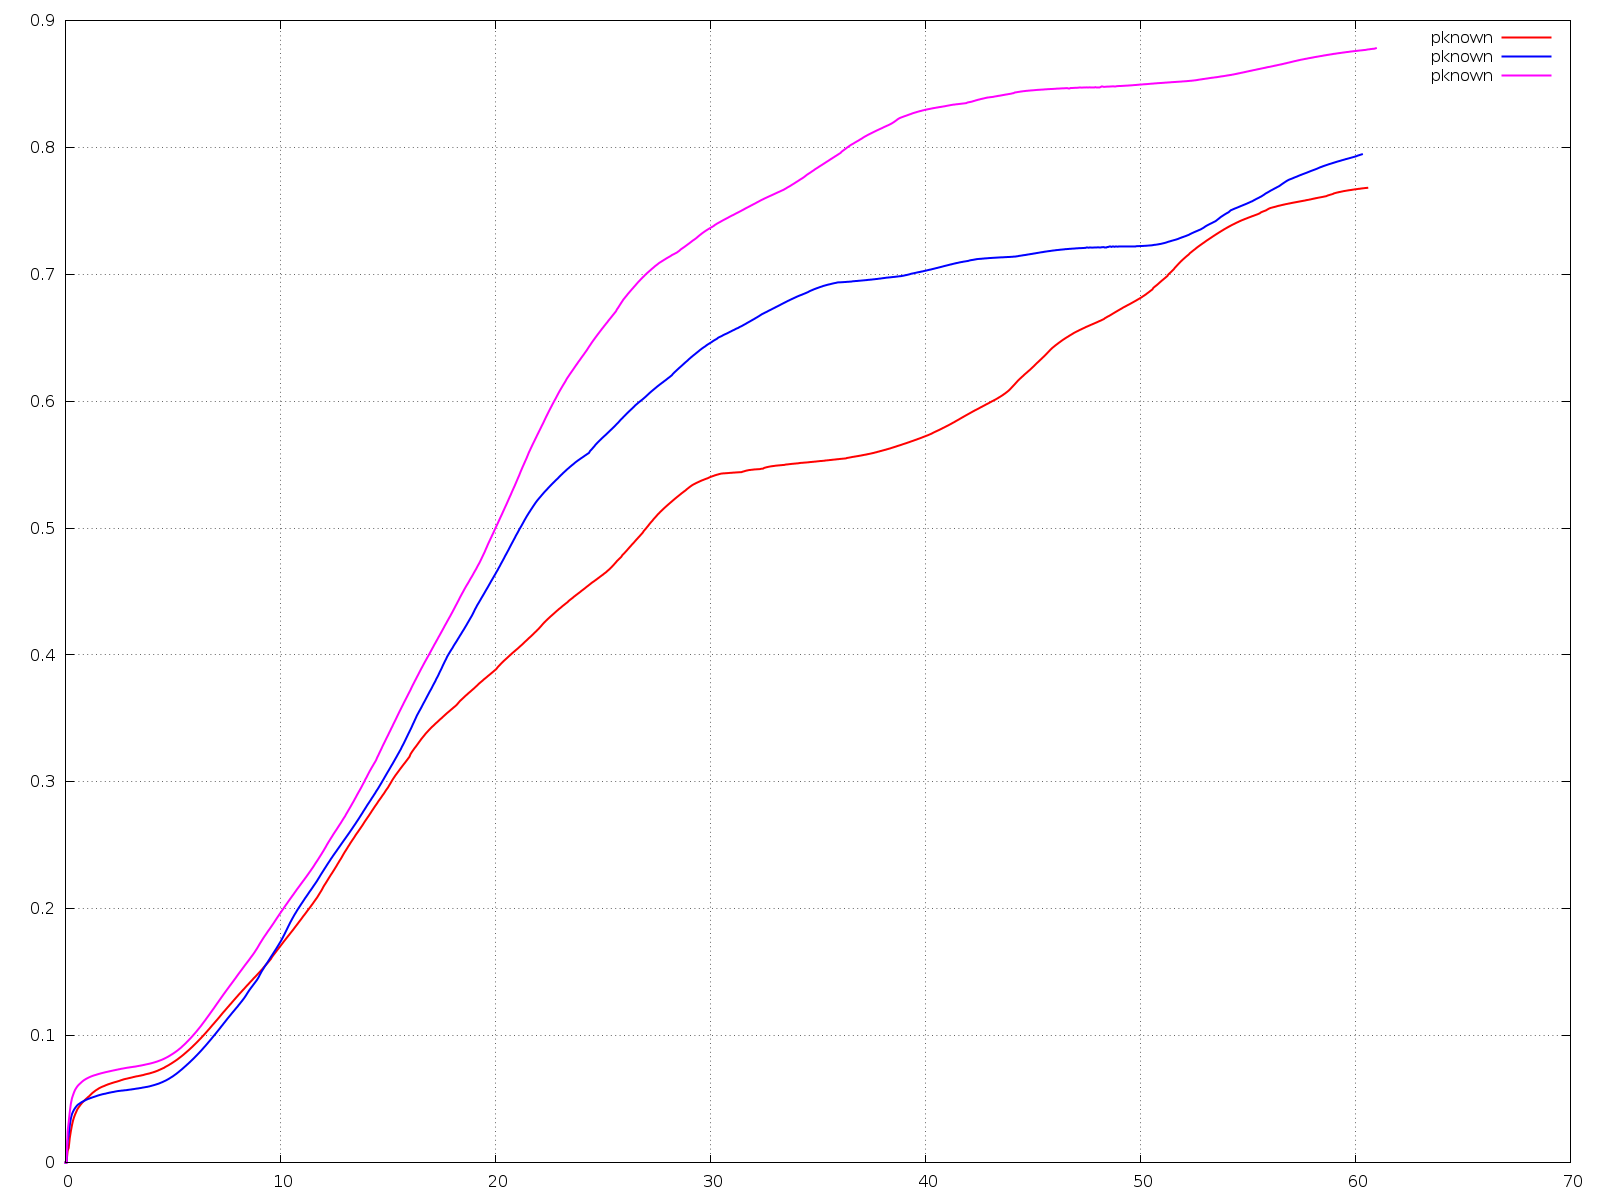
\includegraphics[width=\linewidth]{all_rnd_auto_pknown.png}
    \caption{Случайное перемещение, 3 эксперимента, количество изведанных секторов от времени}
\end{figure}

\begin{figure}[h!]
    \centering
    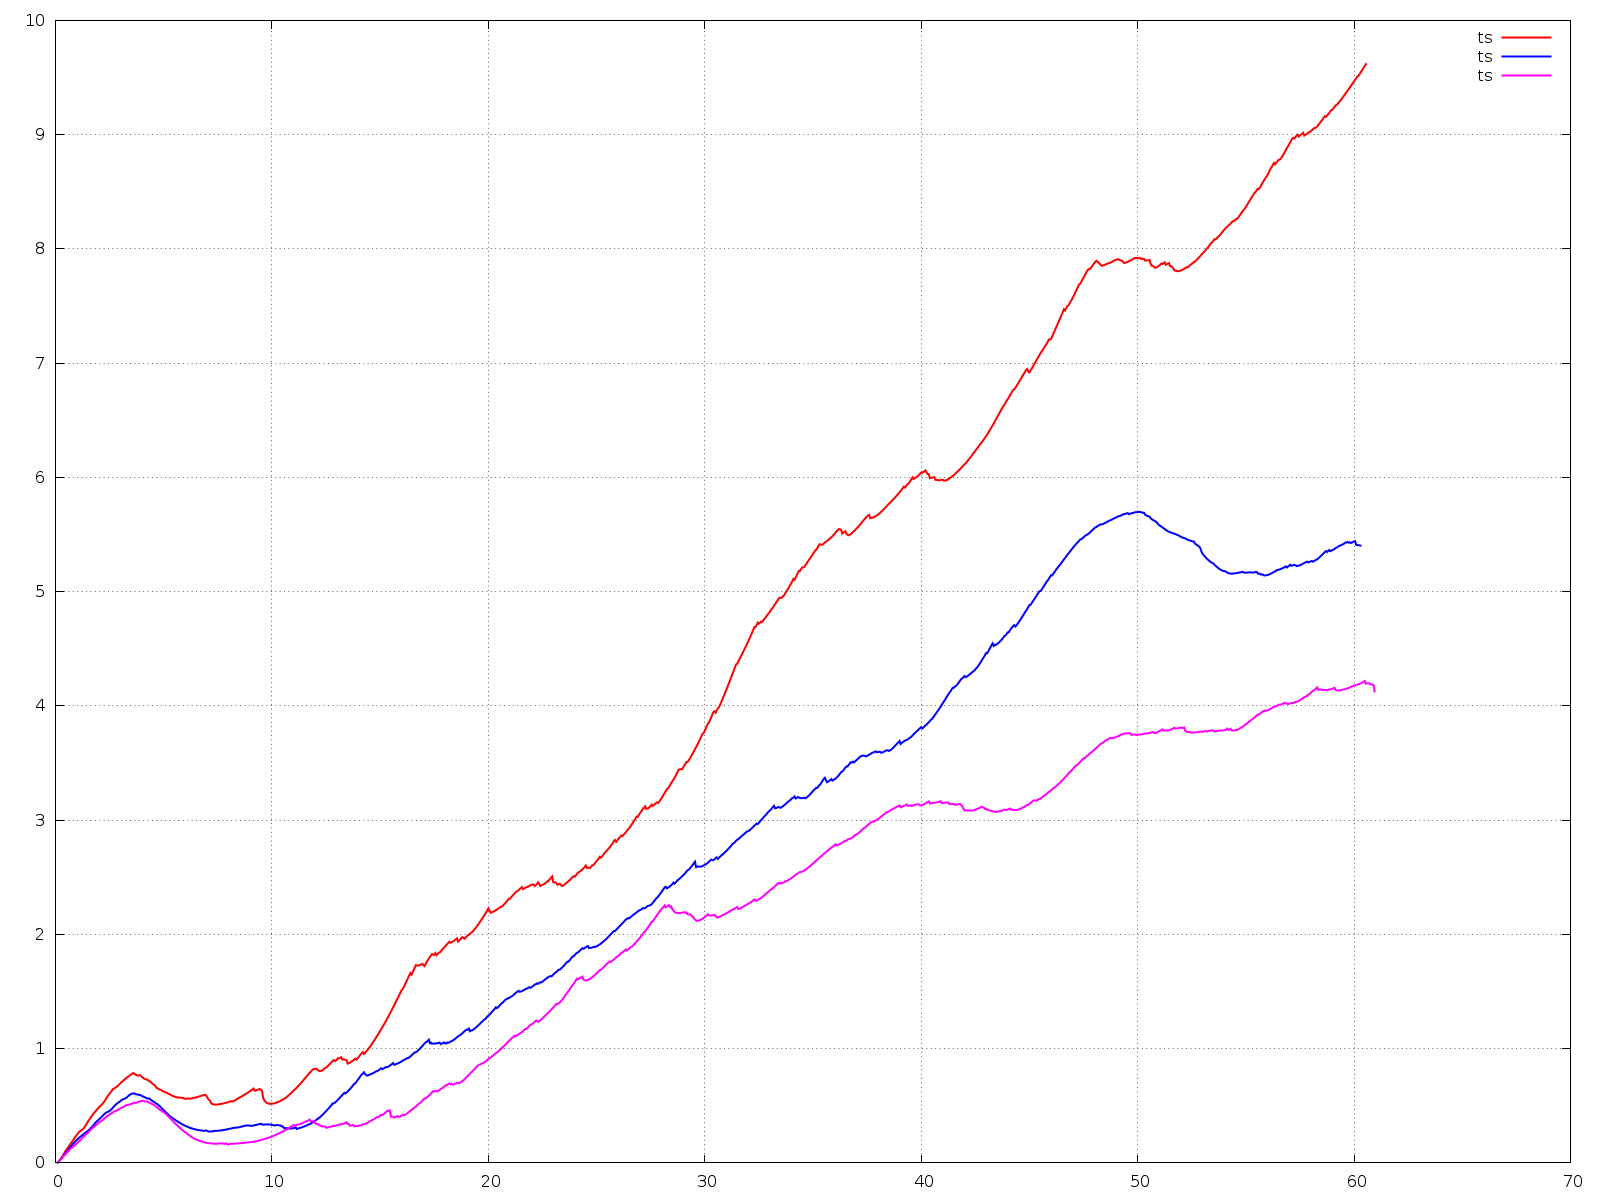
\includegraphics[width=\linewidth]{all_rnd_auto_ts.png}
    \caption{Случайное перемещение, 3 эксперимента, "устаревание" секторов от времени}
\end{figure}

\clearpage
\newpage

\subsubsection{Поиск ближайших неизведанных зон}

\begin{figure}[h!]
    \centering
    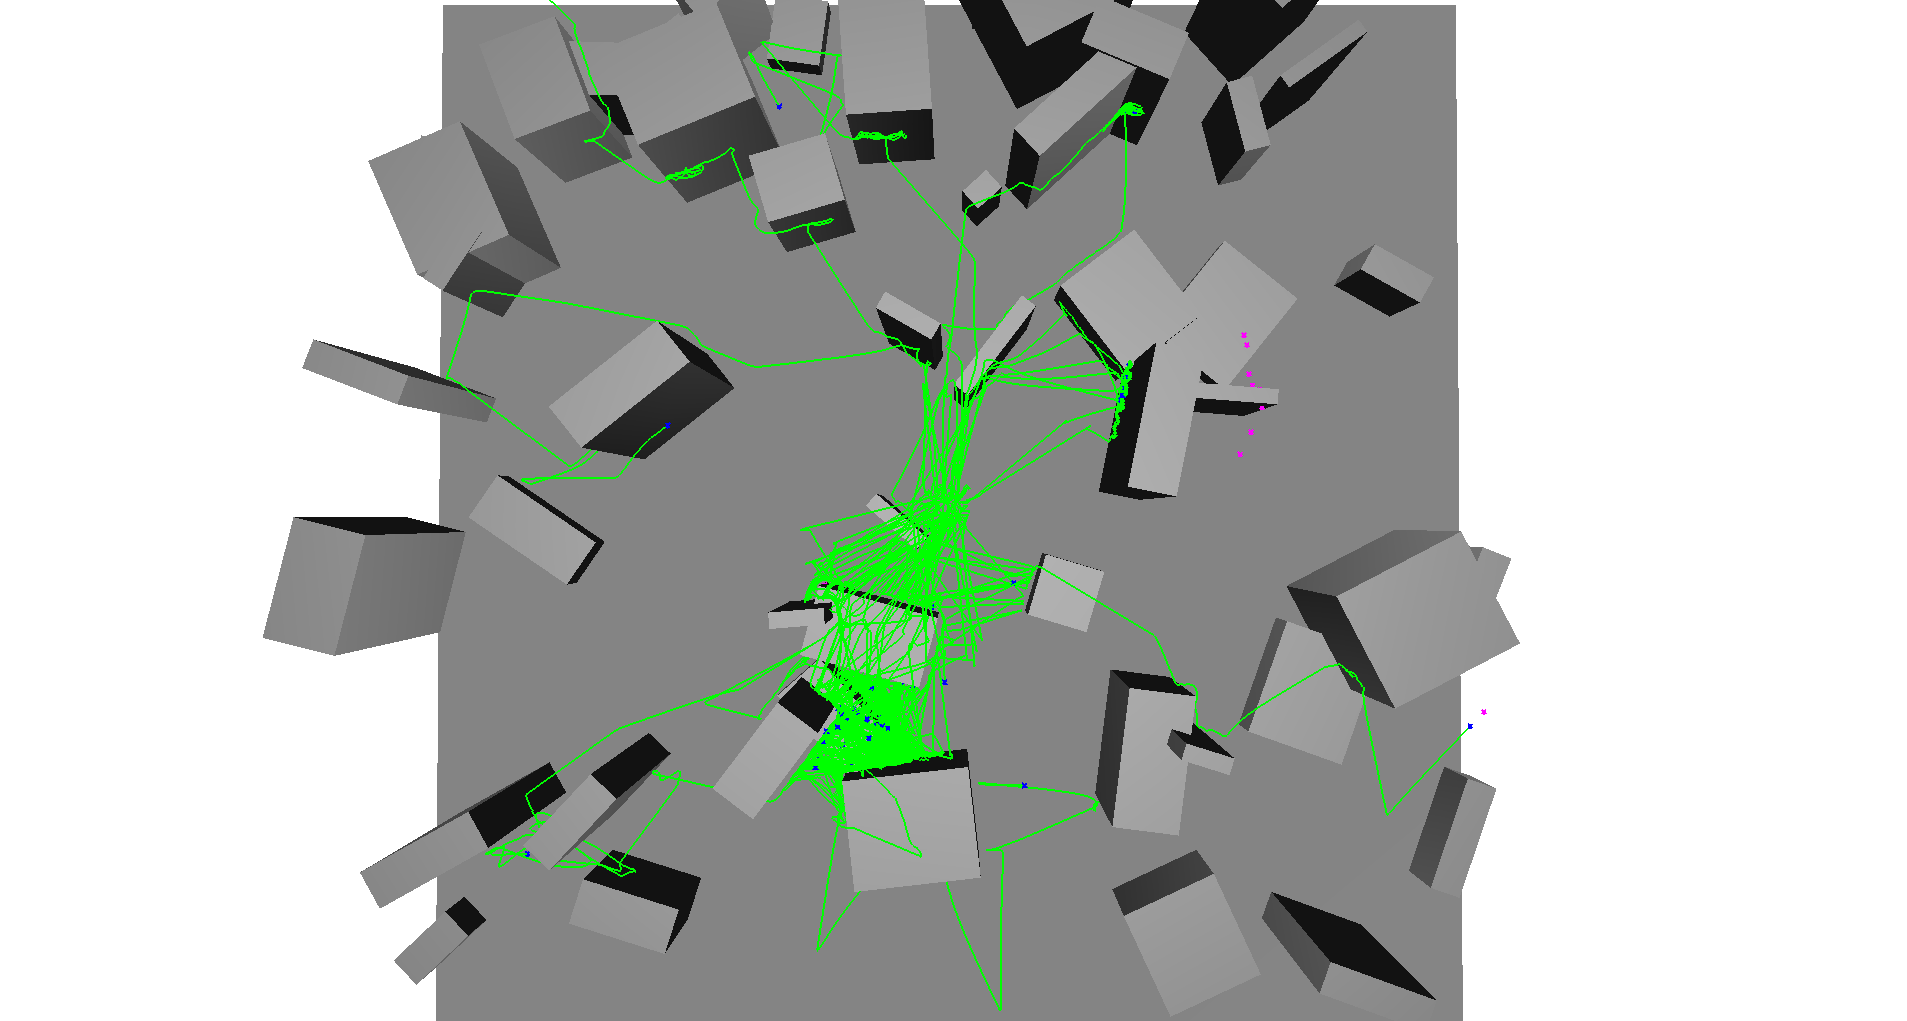
\includegraphics[width=\linewidth]{s50f4r_view.png}
    \caption{Поиск ближайших, 50 юнитов, вид сверху, пути перемещения}
\end{figure}

\begin{figure}[h!]
    \centering
    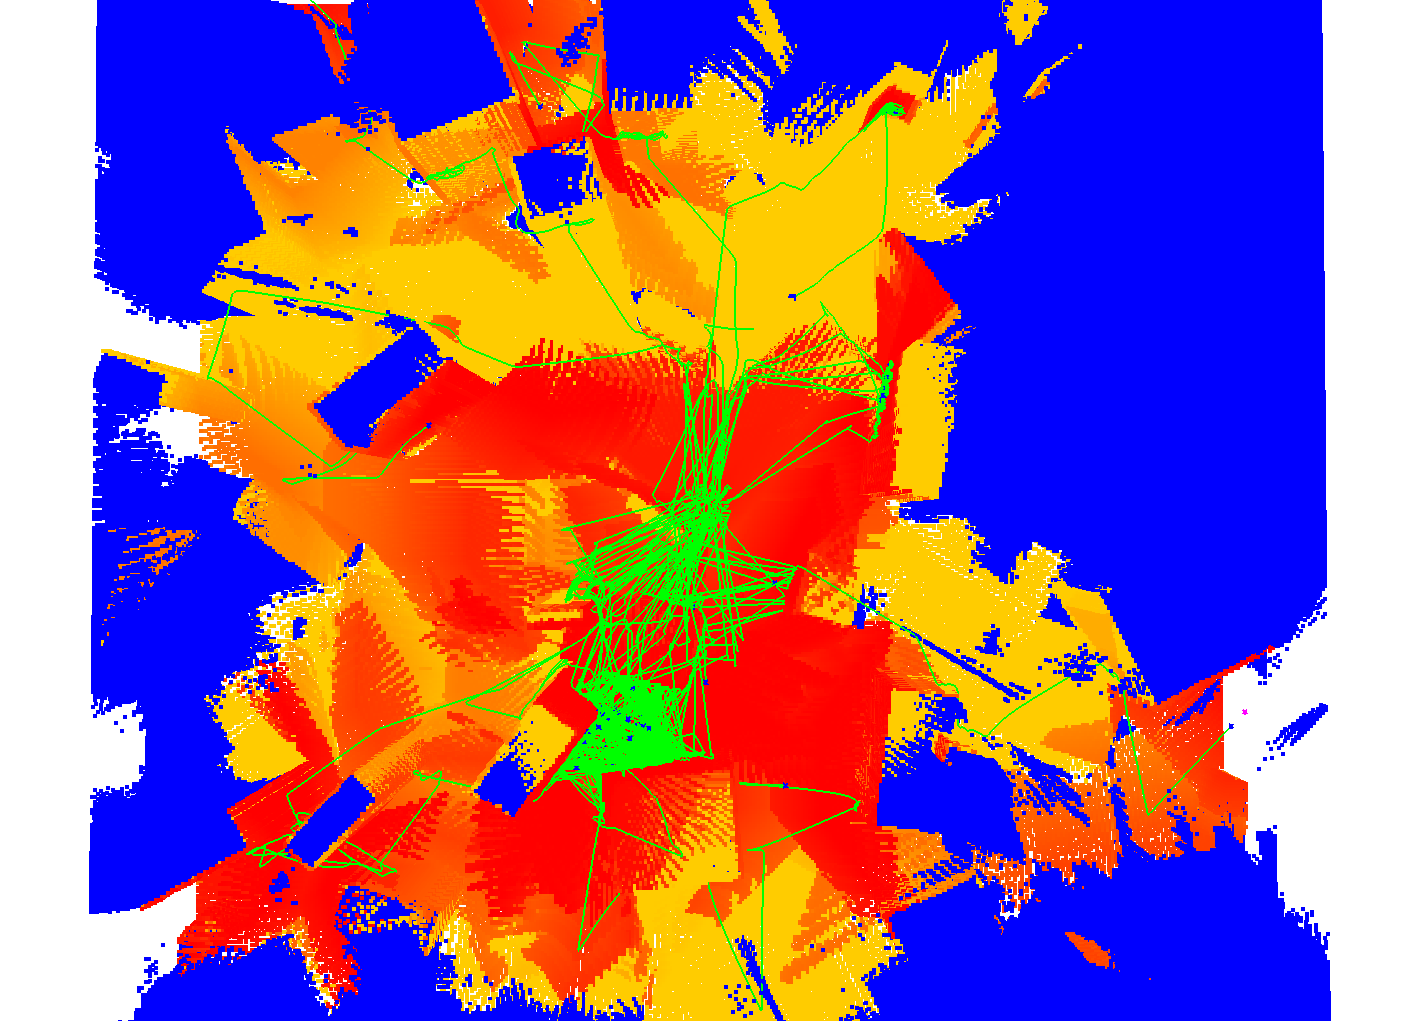
\includegraphics[width=\linewidth]{s50f4r_map.png}
    \caption{Поиск ближайших, 50 юнитов, вид сверху, состояние карты}
\end{figure}

\begin{figure}[h!]
    \centering
    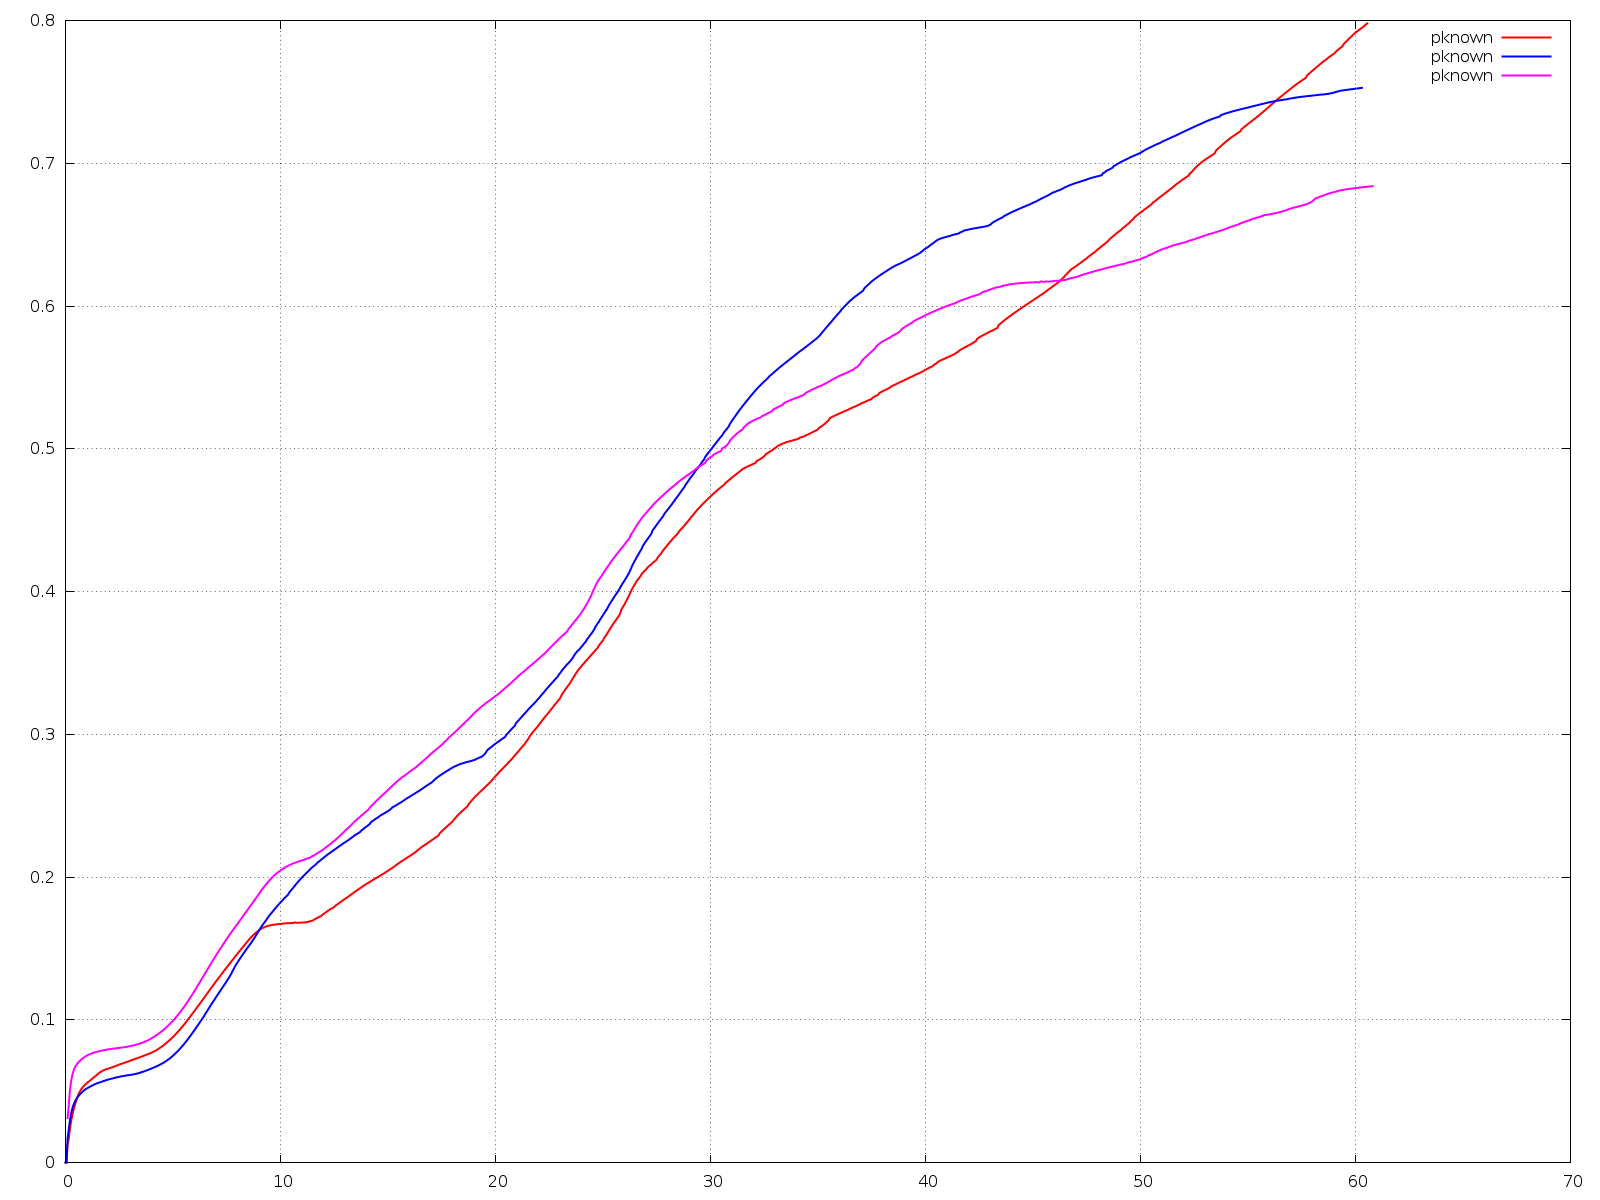
\includegraphics[width=\linewidth]{all_find_4_pknown.png}
    \caption{Поиск ближайших, 3 эксперимента, количество изведанных секторов от времени}
\end{figure}

\begin{figure}[h!]
    \centering
    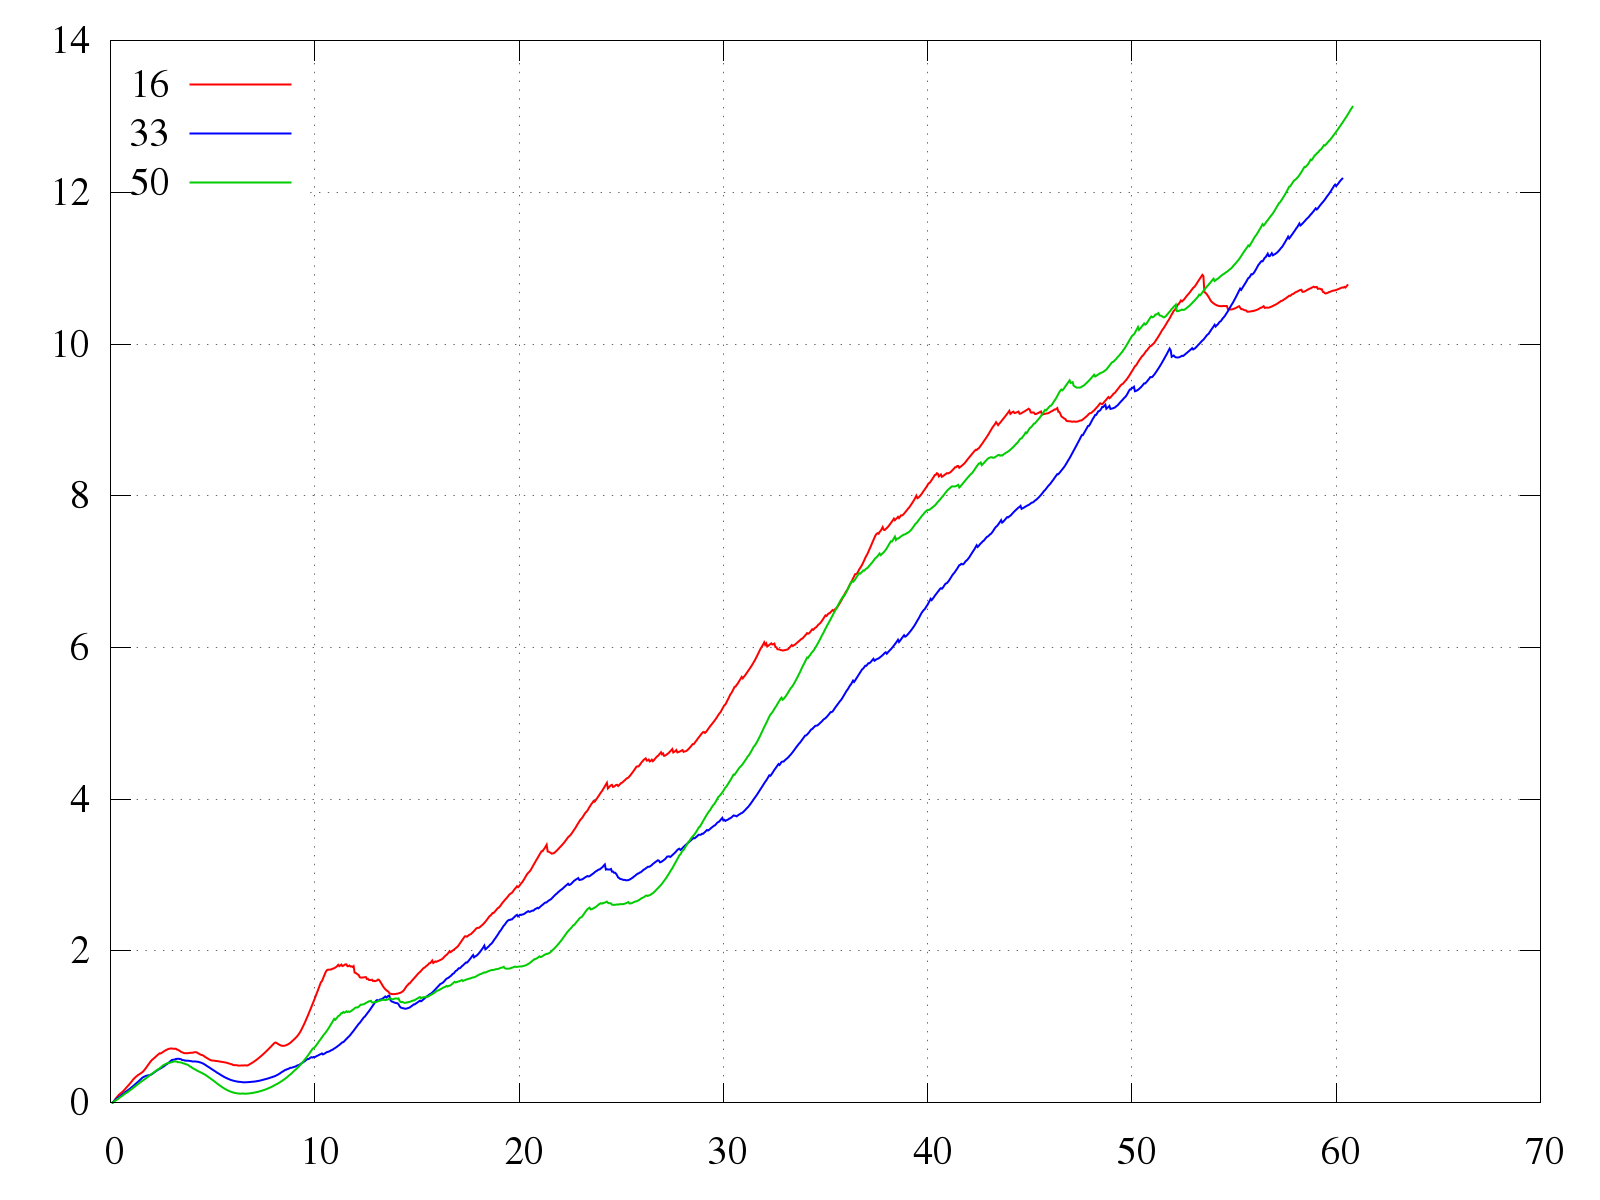
\includegraphics[width=\linewidth]{all_find_4_ts.png}
    \caption{Поиск ближайших, 3 эксперимента, "устаревание" секторов от времени}
\end{figure}

\clearpage
\newpage

\subsubsection{Равномерное распределение по карте}

\begin{figure}[h!]
    \centering
    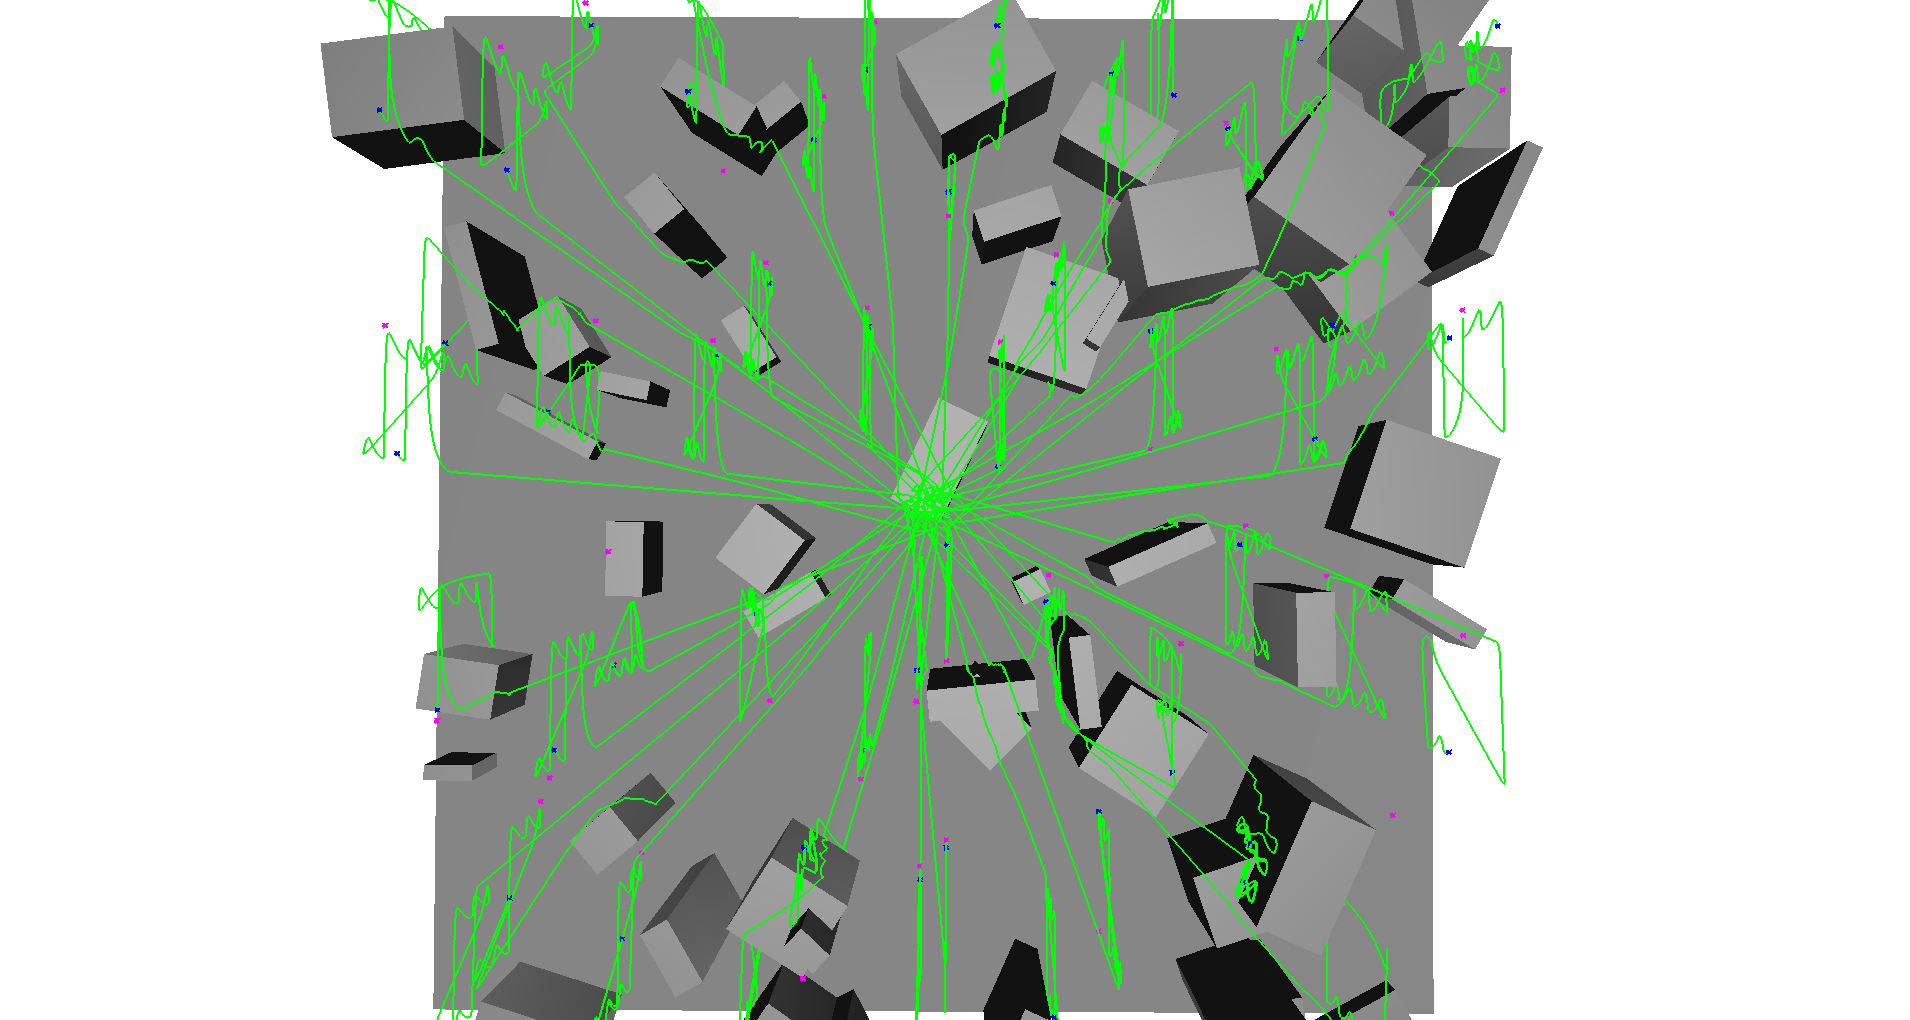
\includegraphics[width=\linewidth]{s50s_view.png}
    \caption{Равномерное распределение, 50 юнитов, вид сверху, пути перемещения}
\end{figure}

\begin{figure}[h!]
    \centering
    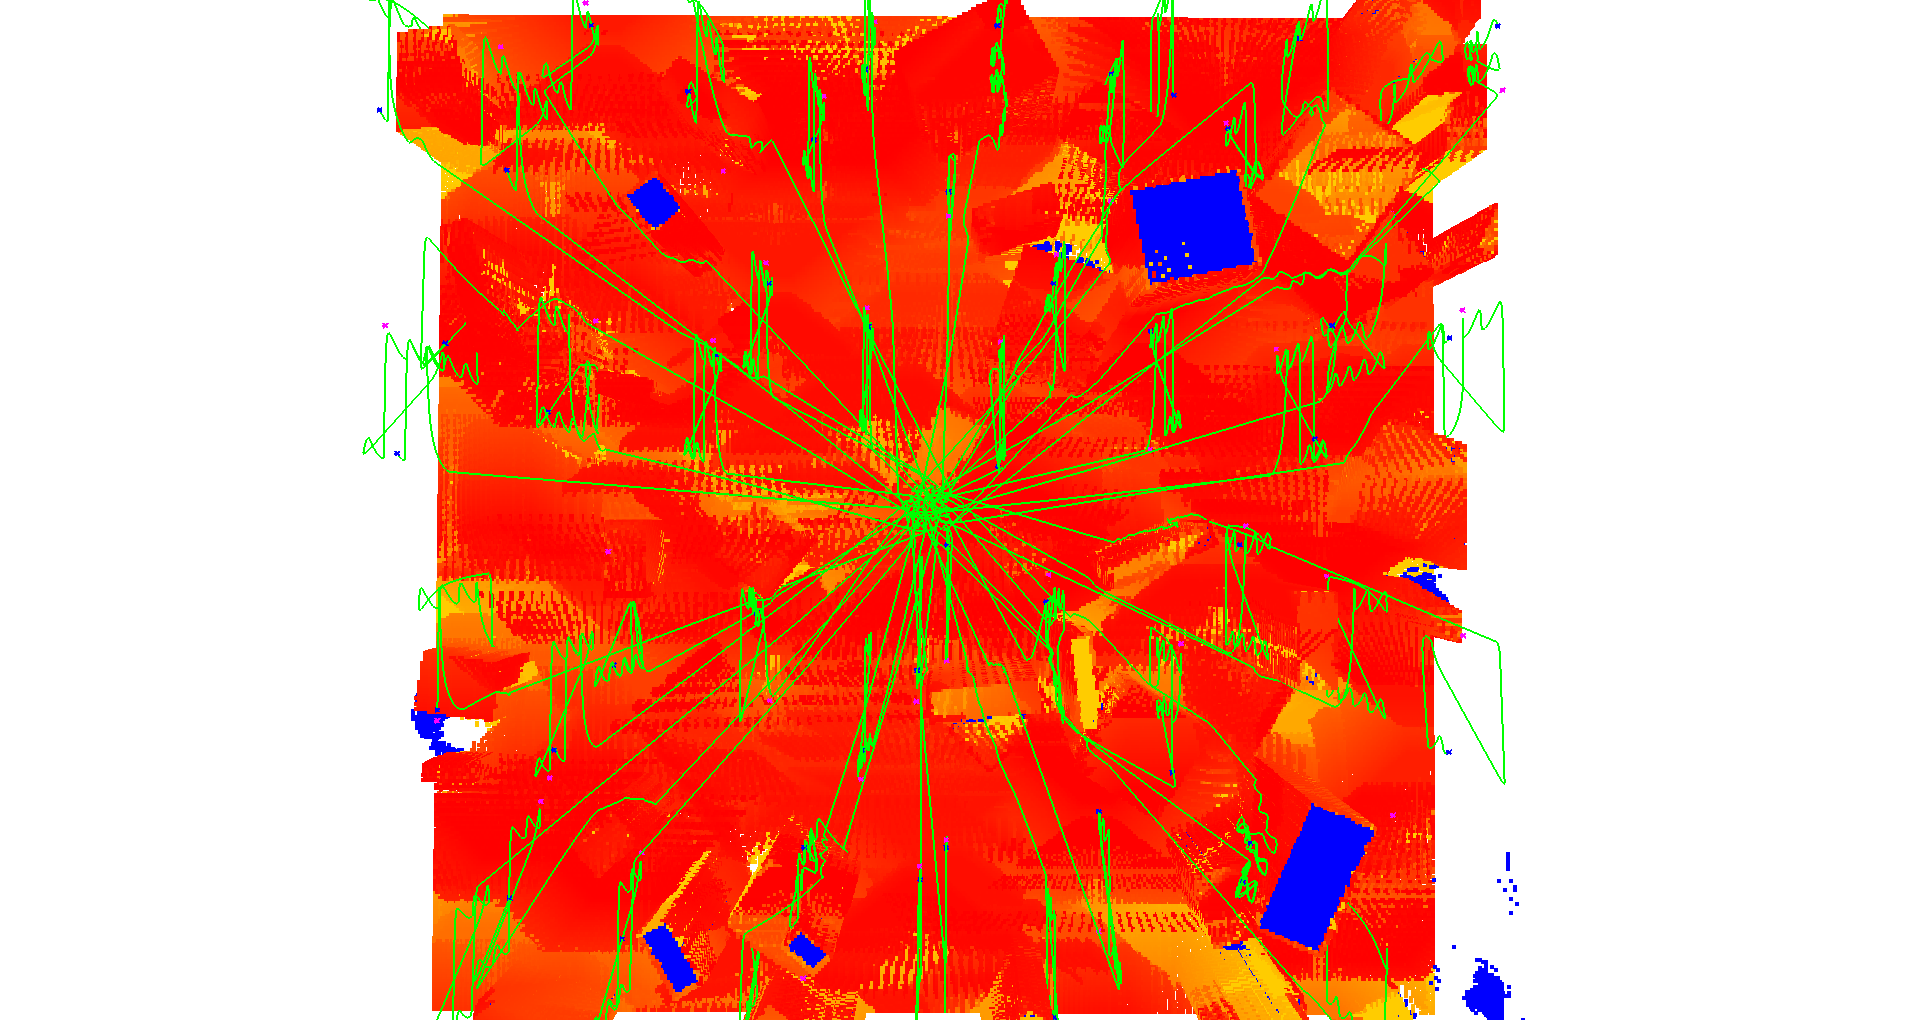
\includegraphics[width=\linewidth]{s50s_map1.png}
    \caption{Равномерное распределение, 50 юнитов, вид сверху, состояние карты}
\end{figure}

\begin{figure}[h!]
    \centering
    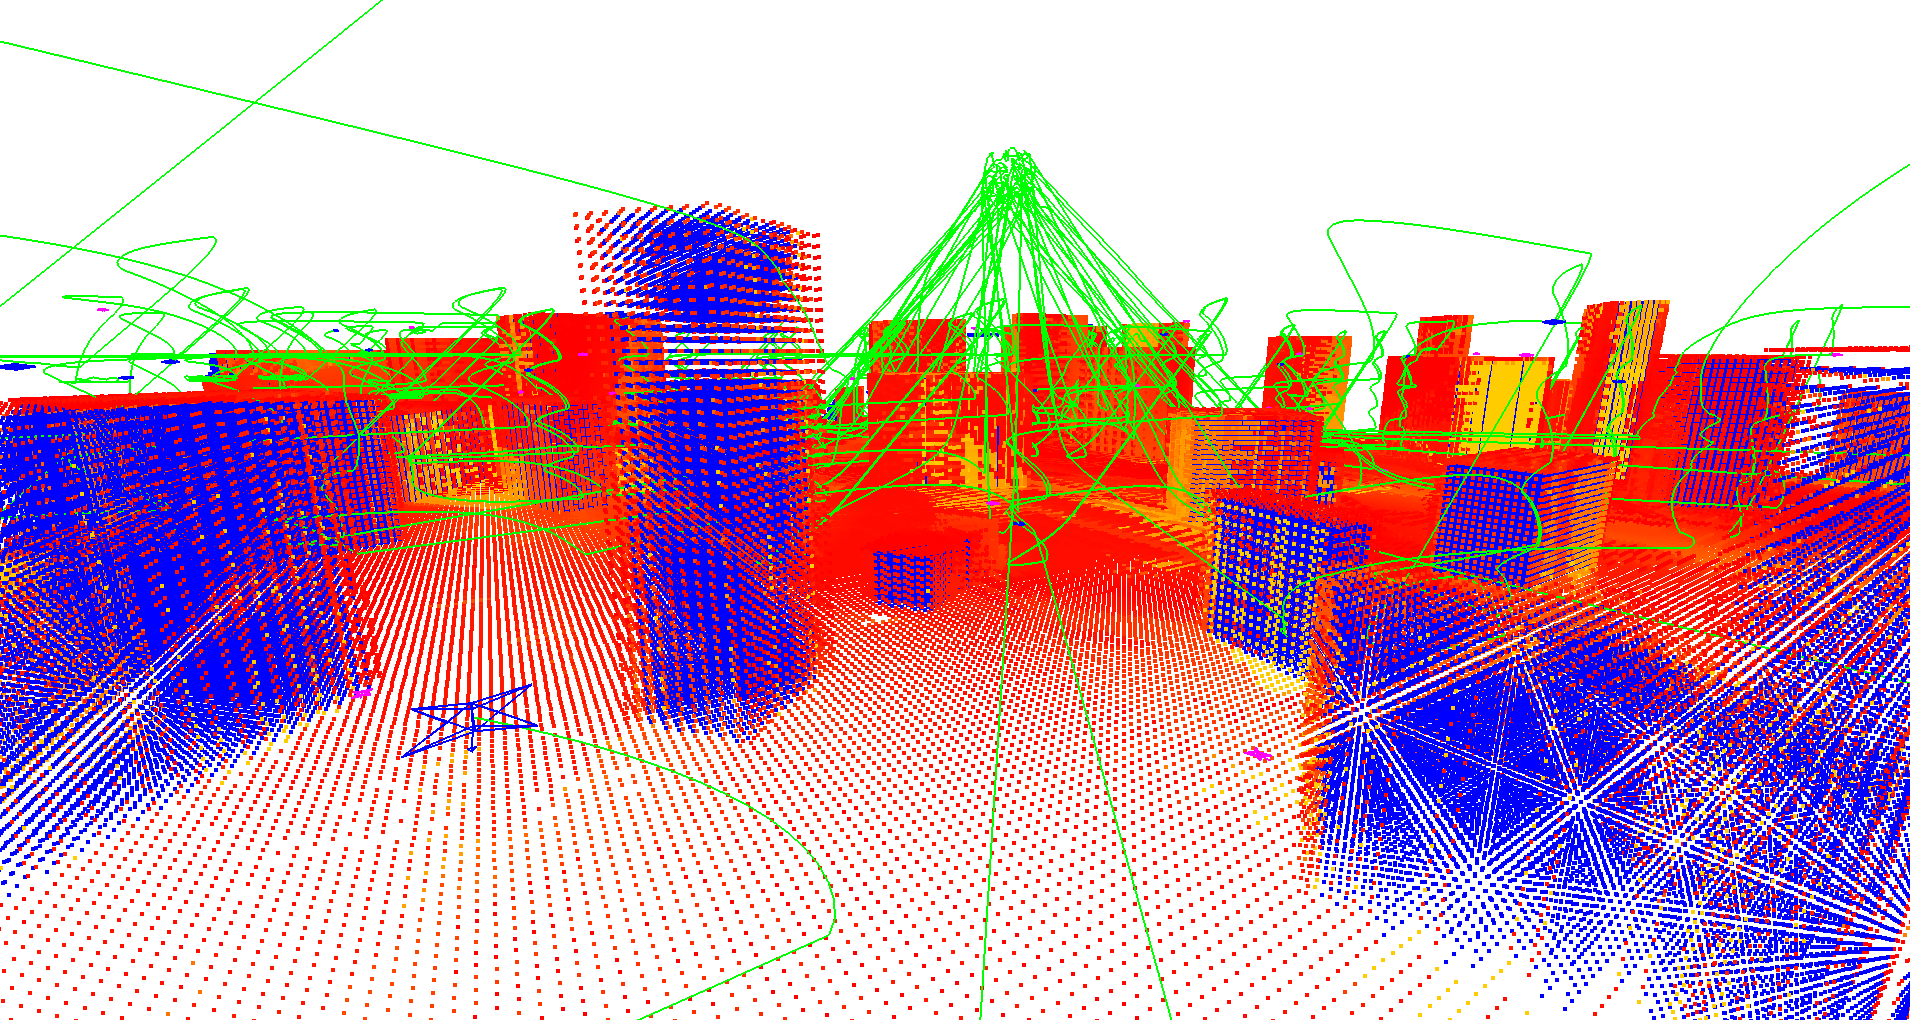
\includegraphics[width=\linewidth]{s50s_map2.png}
    \caption{Равномерное распределение, 50 юнитов, вид сбоку, состояние карты}
\end{figure}

\begin{figure}[h!]
    \centering
    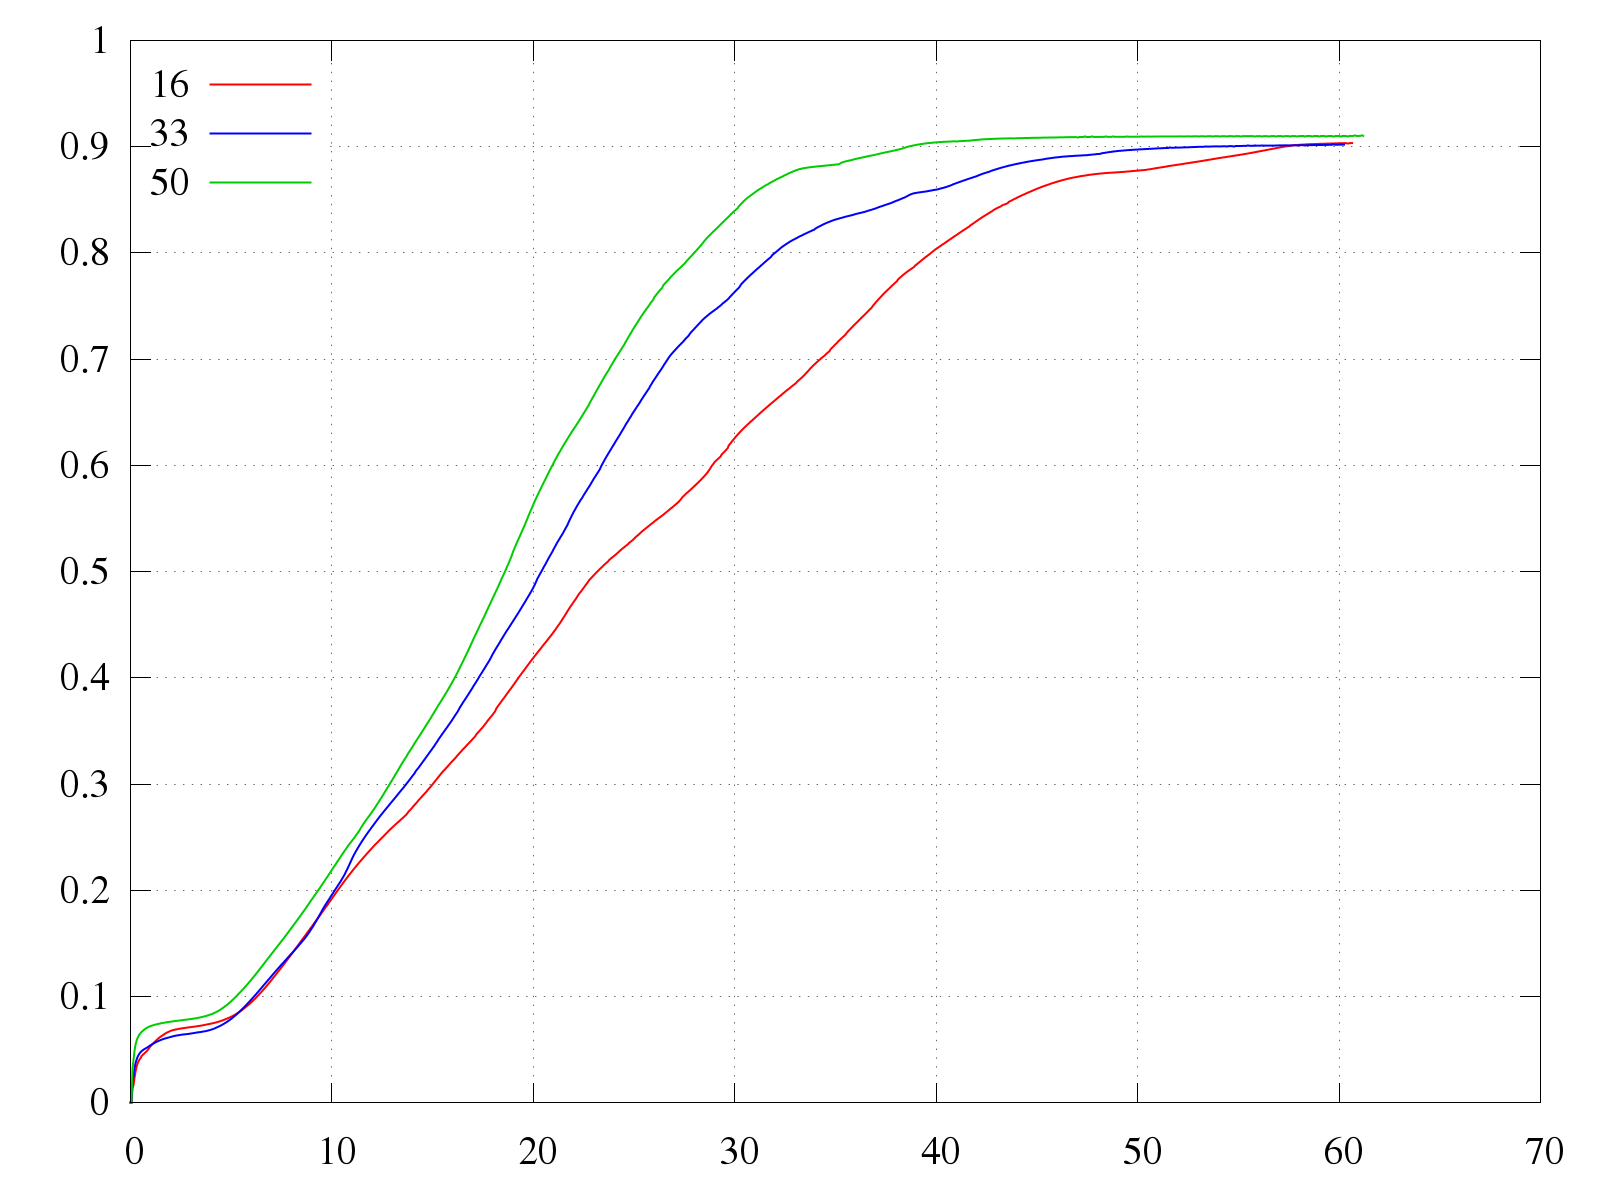
\includegraphics[width=\linewidth]{all_serial_pknown.png}
    \caption{Равномерное распределение, 3 эксперимента, количество изведанных секторов от времени}
\end{figure}

\begin{figure}[h!]
    \centering
    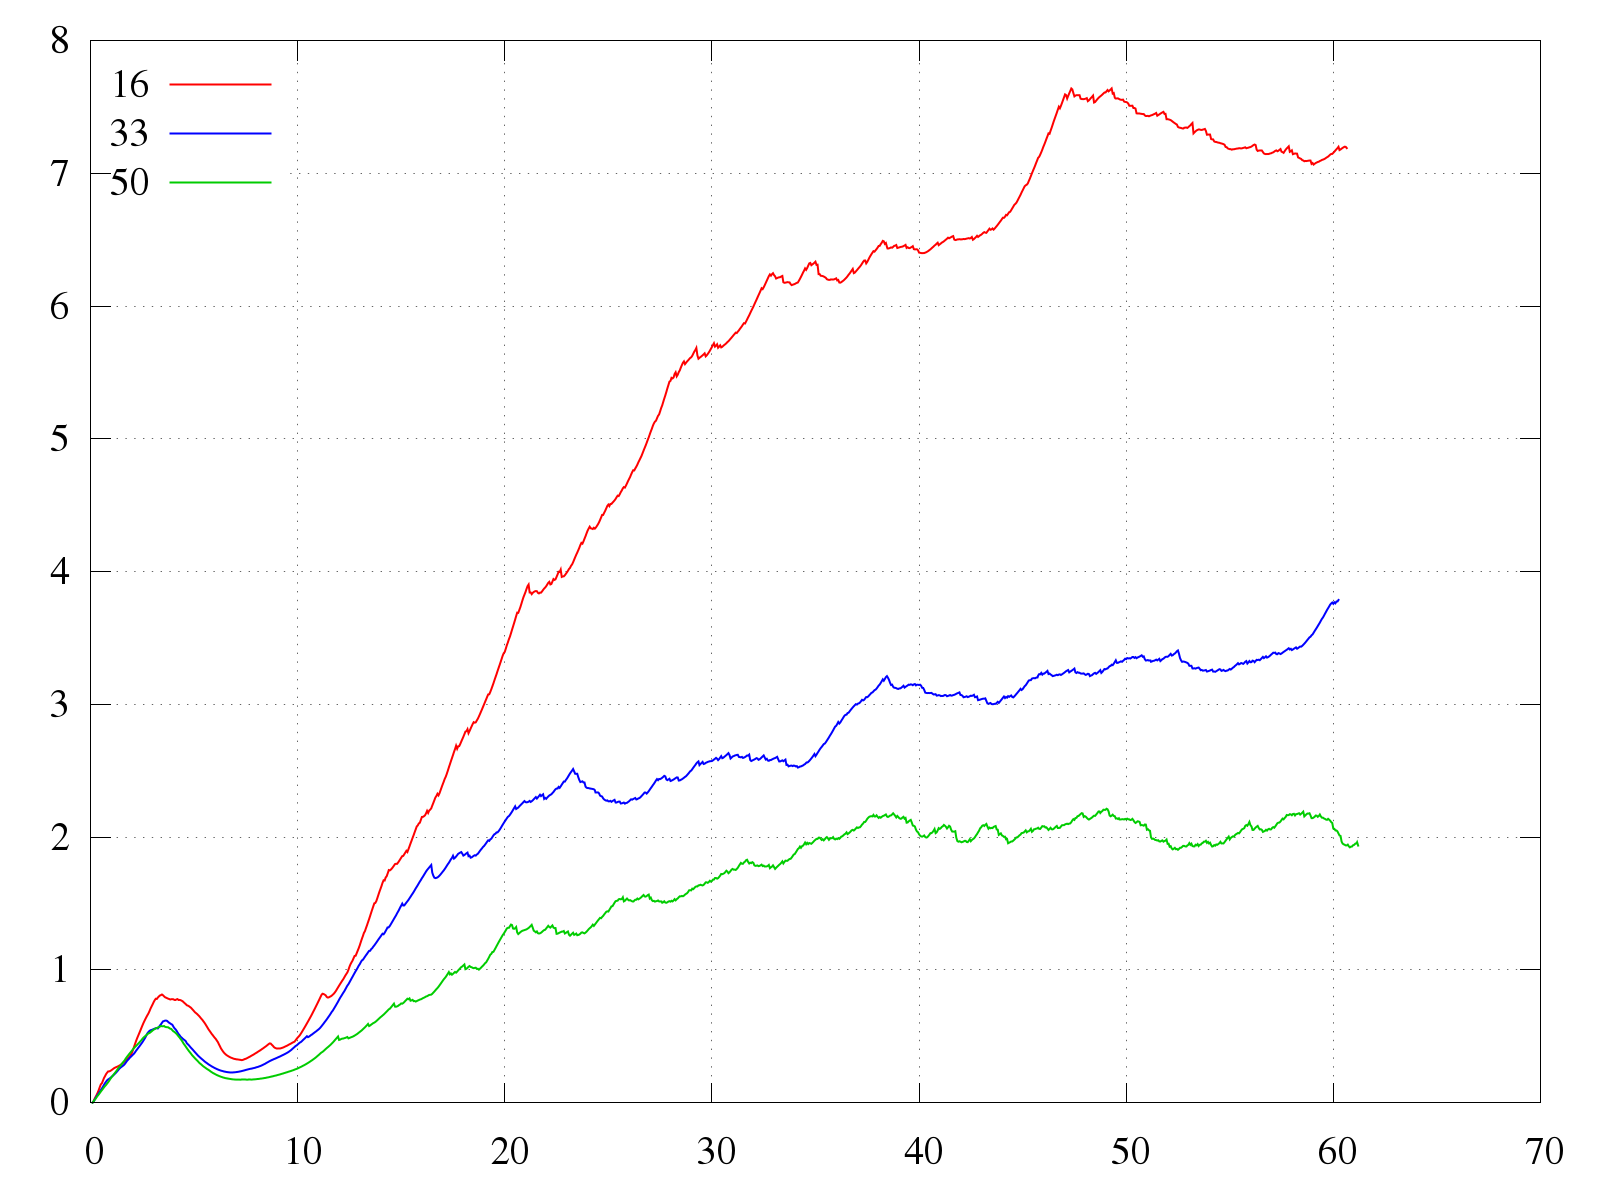
\includegraphics[width=\linewidth]{all_serial_ts.png}
    \caption{Равномерное распределение, 3 эксперимента, "устаревание" секторов от времени}
\end{figure}

\clearpage
\newpage

\subsubsection{Сравнение алгоритмов}

\begin{figure}[h!]
    \centering
    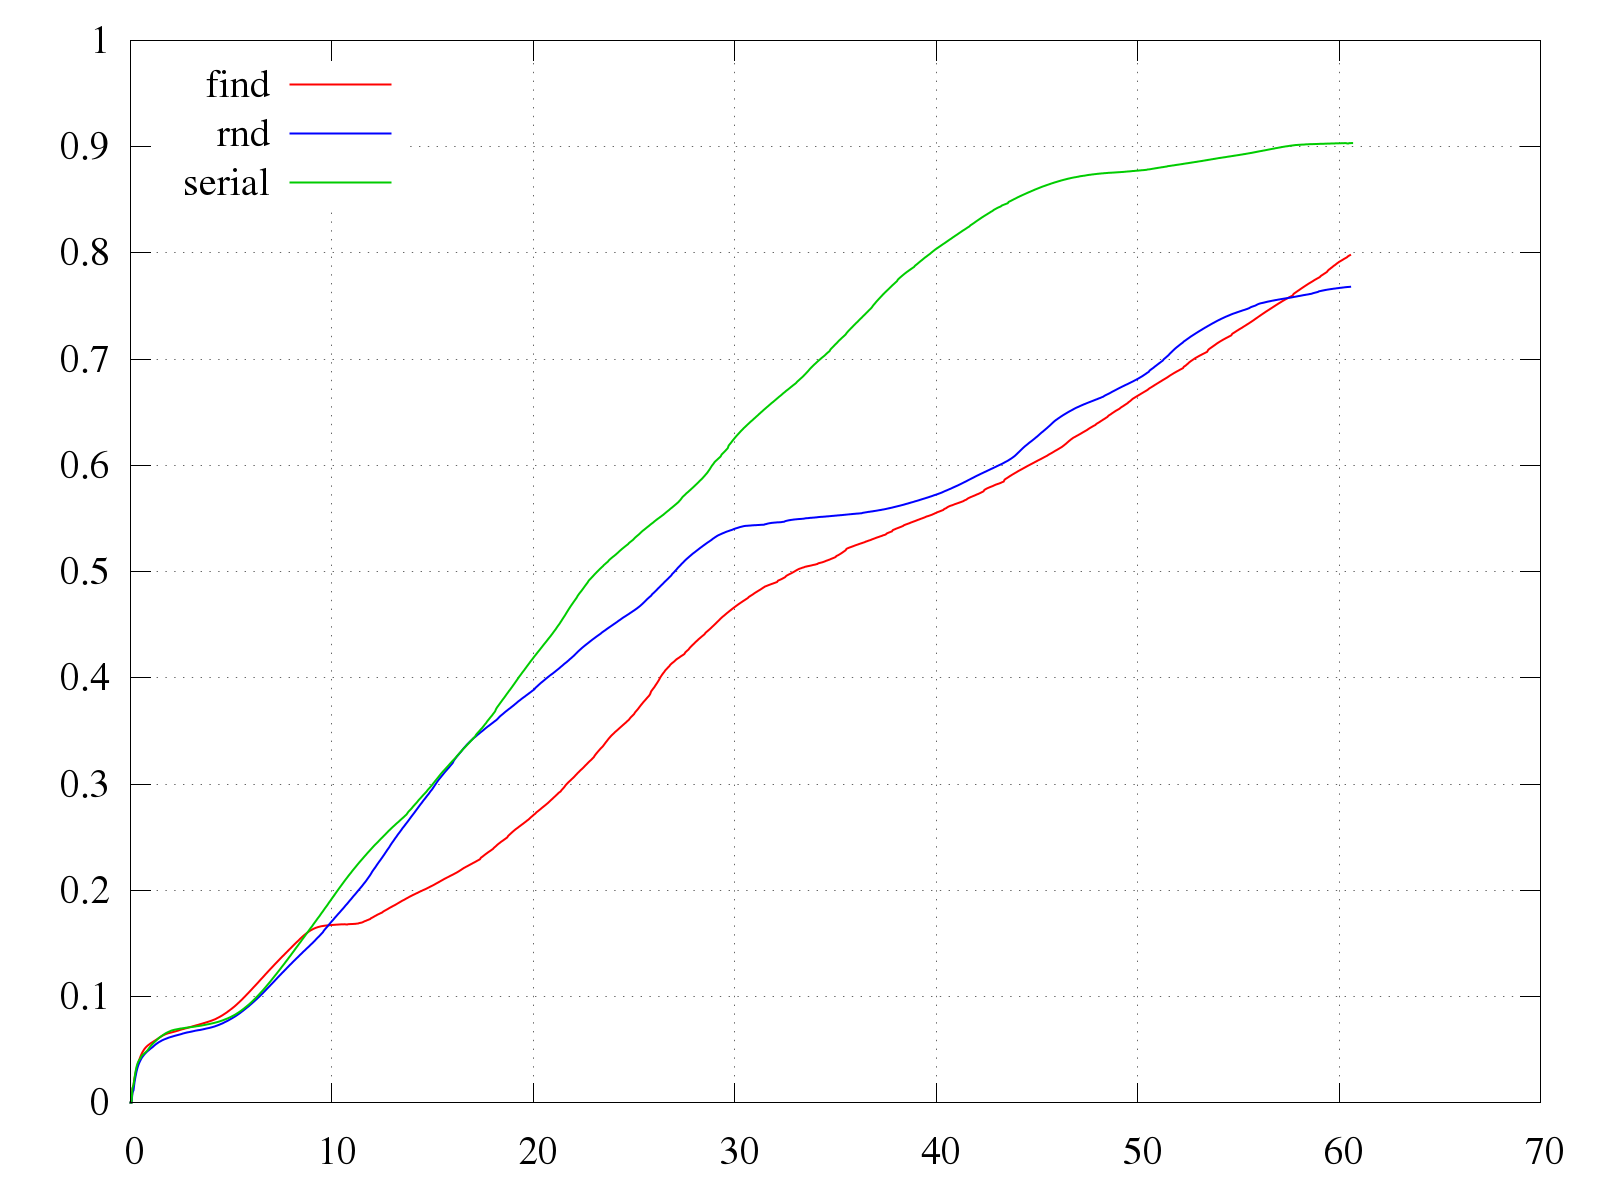
\includegraphics[width=\linewidth]{all_16_pknown.png}
    \caption{3 алгоритма, 16 юнитов, количество изведанных секторов от времени}
\end{figure}

\begin{figure}[h!]
    \centering
    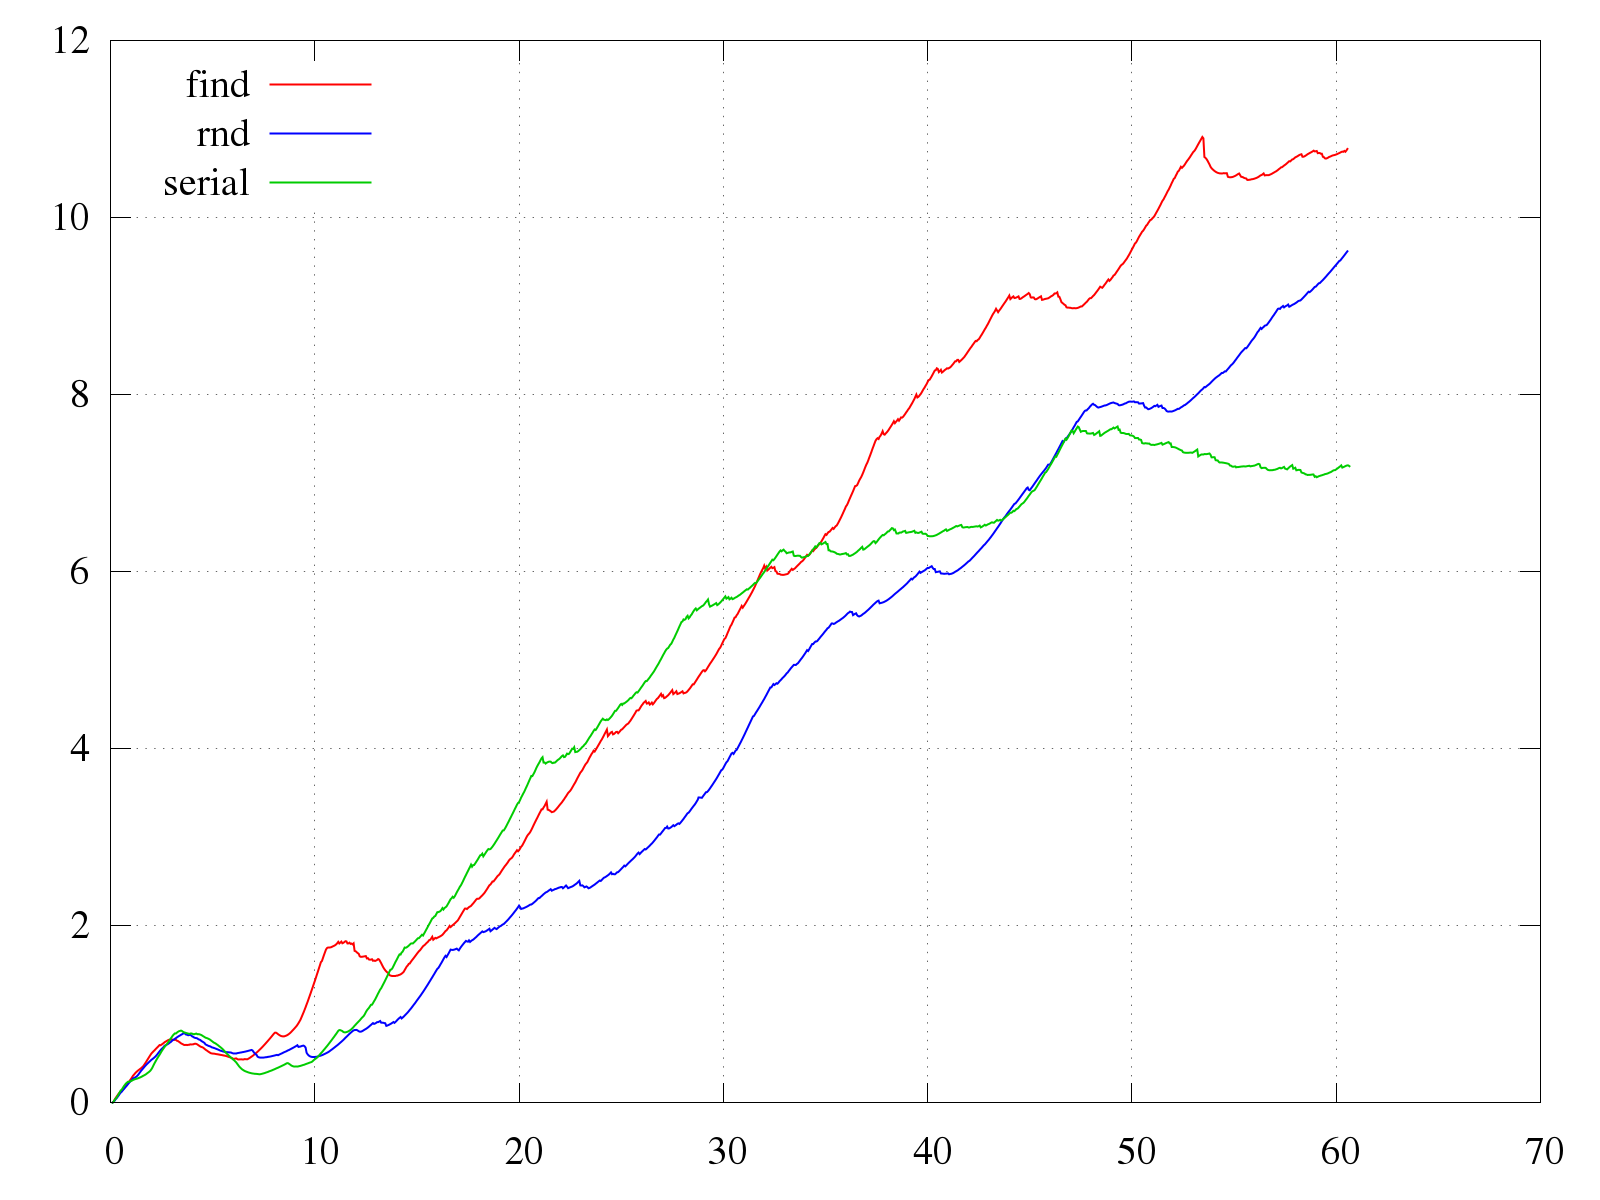
\includegraphics[width=\linewidth]{all_16_ts.png}
    \caption{3 алгоритма, 16 юнитов, "устаревание" секторов от времени}
\end{figure}

\begin{figure}[h!]
    \centering
    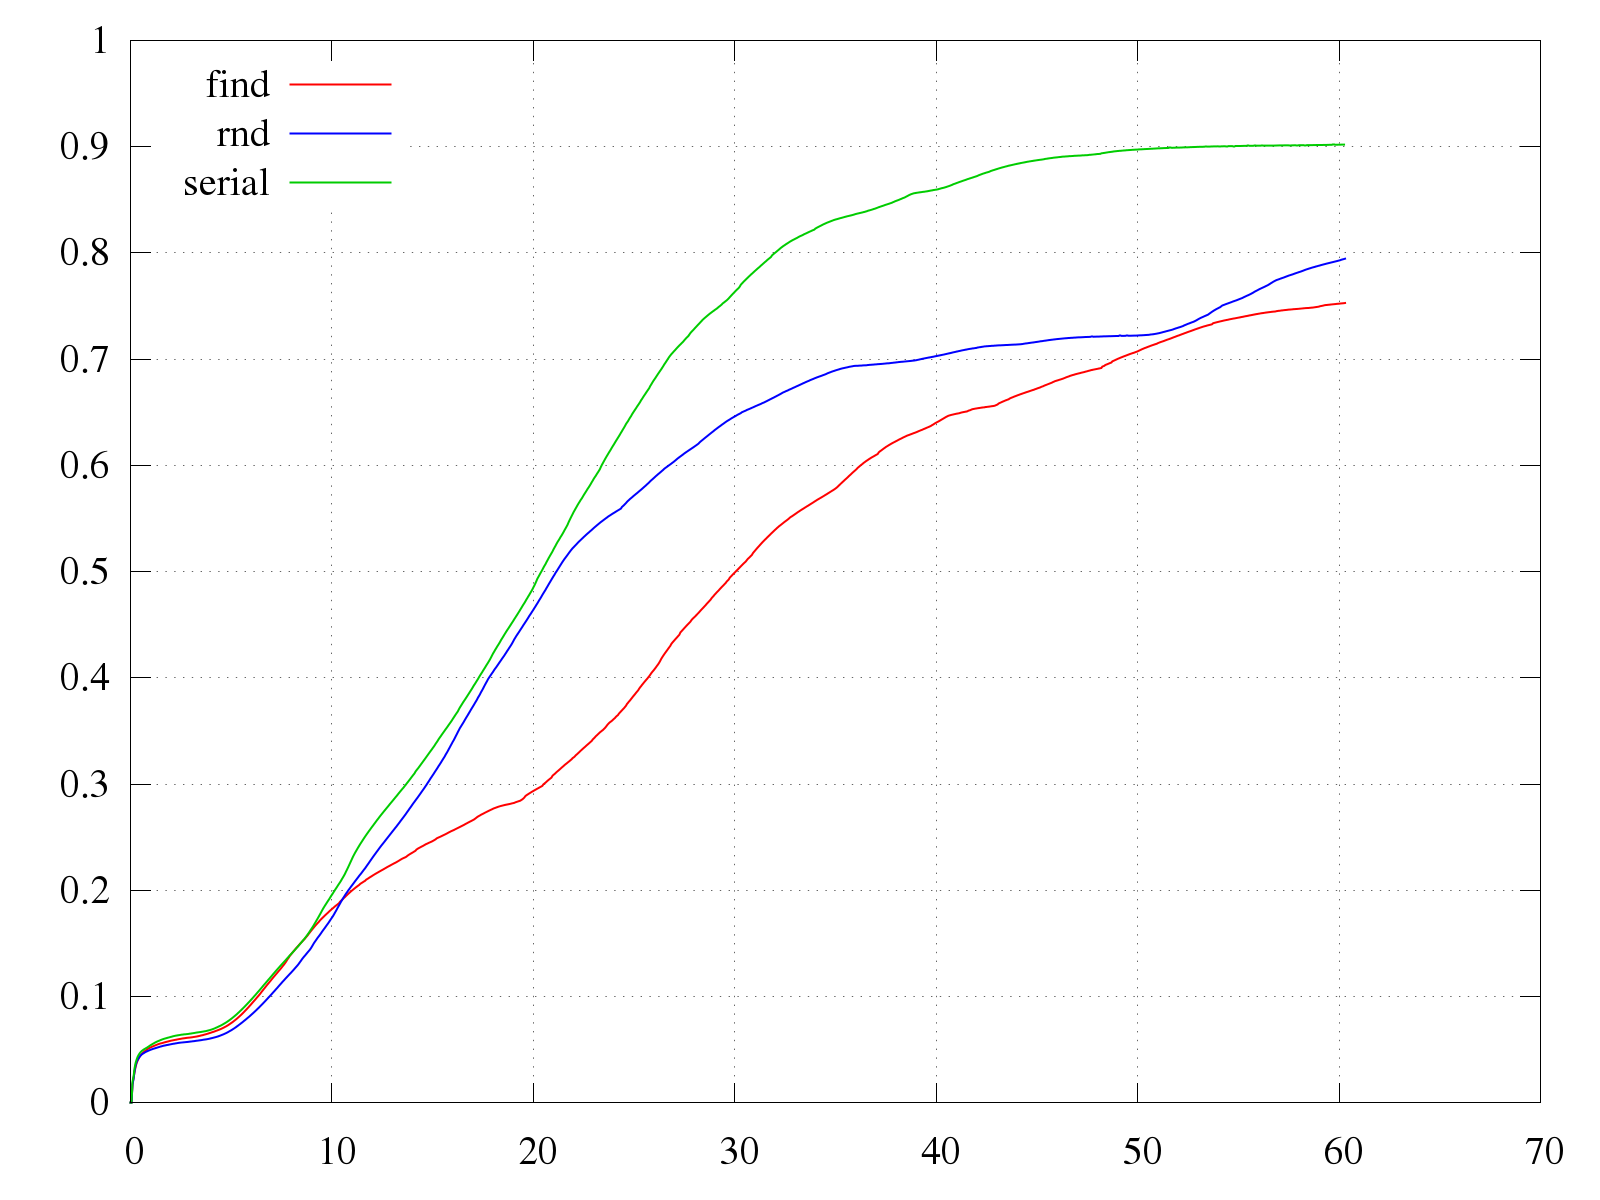
\includegraphics[width=\linewidth]{all_33_pknown.png}
    \caption{3 алгоритма, 33 юнитов, количество изведанных секторов от времени}
\end{figure}

\begin{figure}[h!]
    \centering
    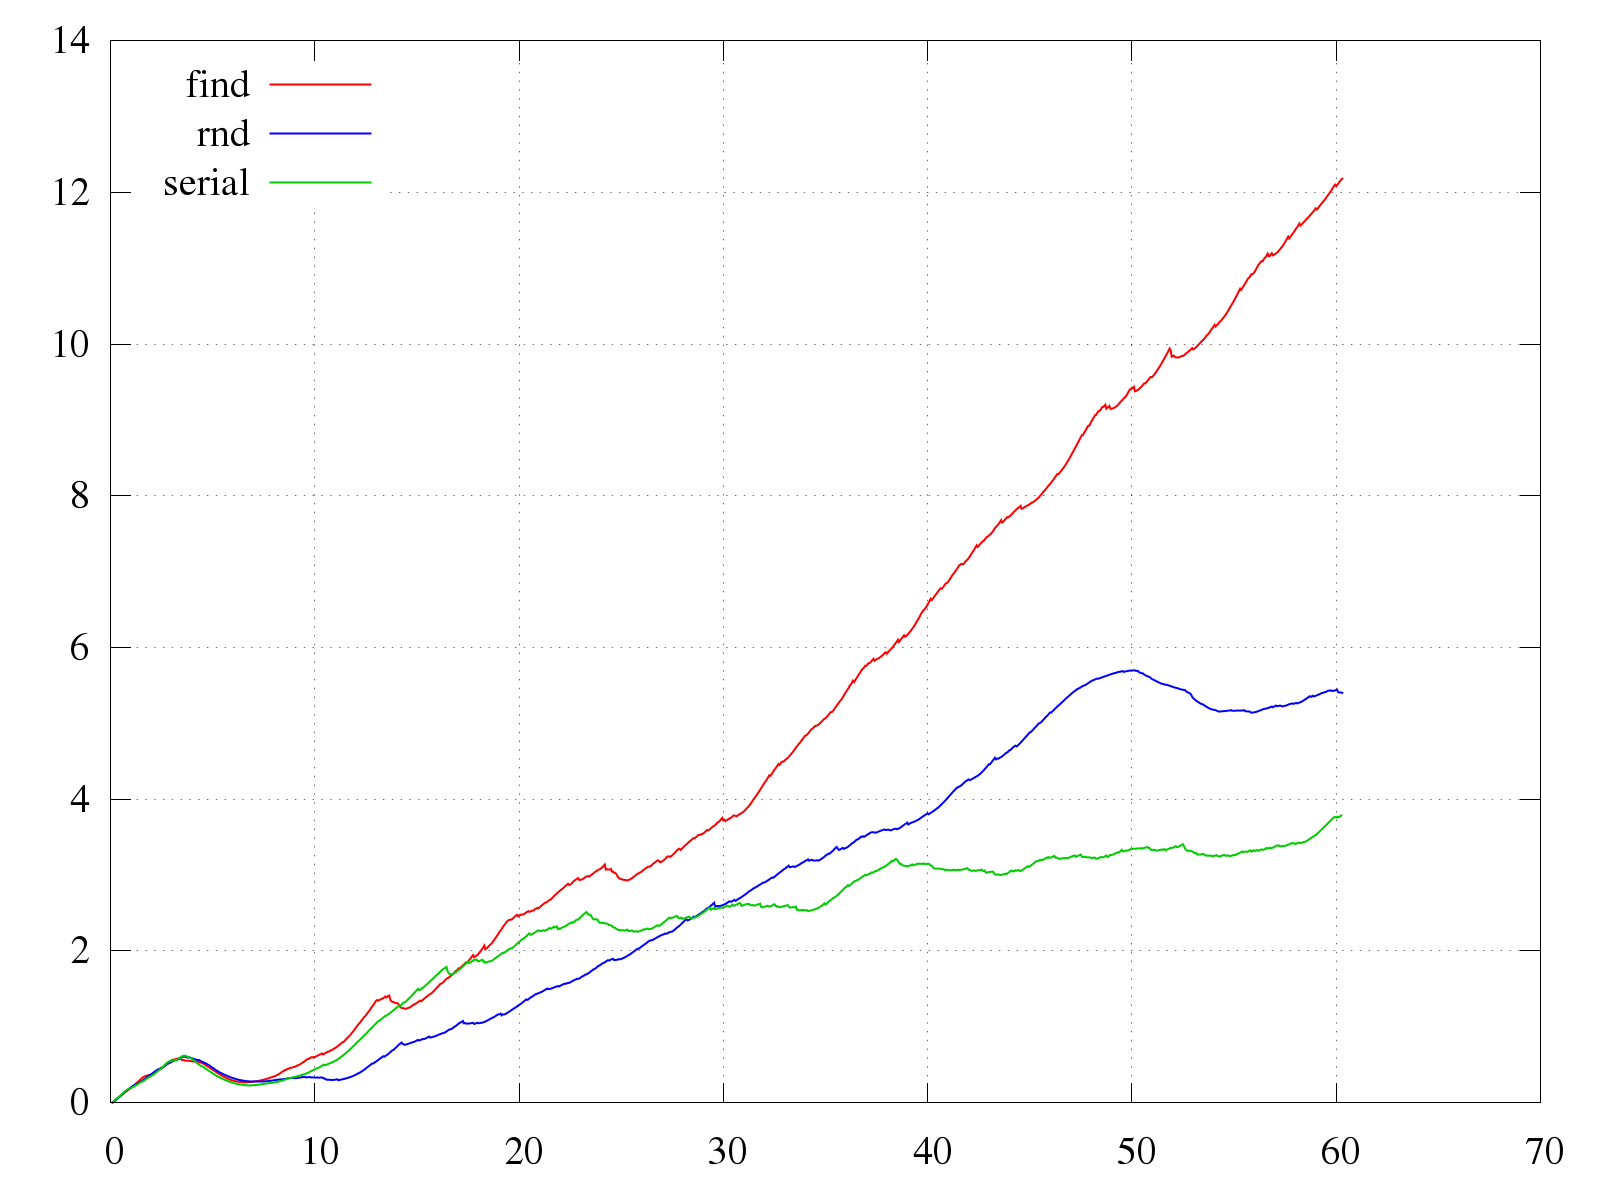
\includegraphics[width=\linewidth]{all_33_ts.png}
    \caption{3 алгоритма, 33 юнитов, "устаревание" секторов от времени}
\end{figure}

\begin{figure}[h!]
    \centering
    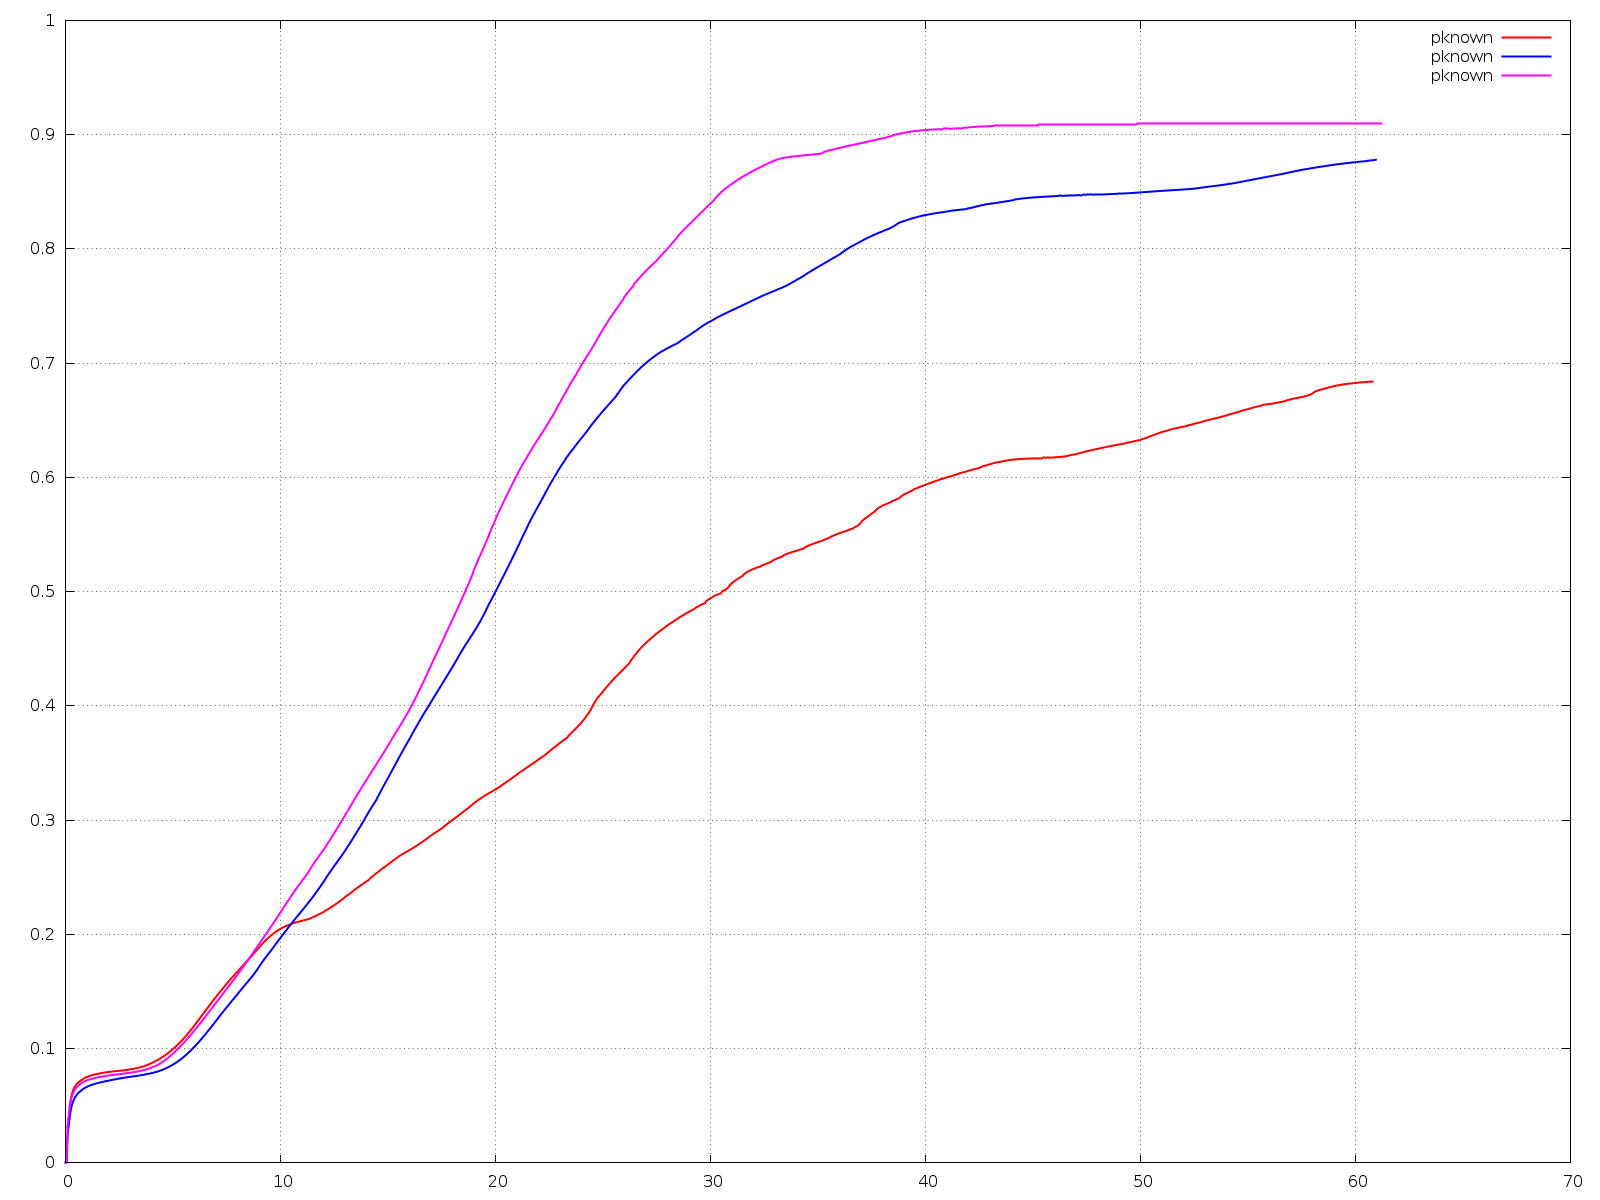
\includegraphics[width=\linewidth]{all_50_pknown.png}
    \caption{3 алгоритма, 50 юнитов, количество изведанных секторов от времени}
\end{figure}

\begin{figure}[h!]
    \centering
    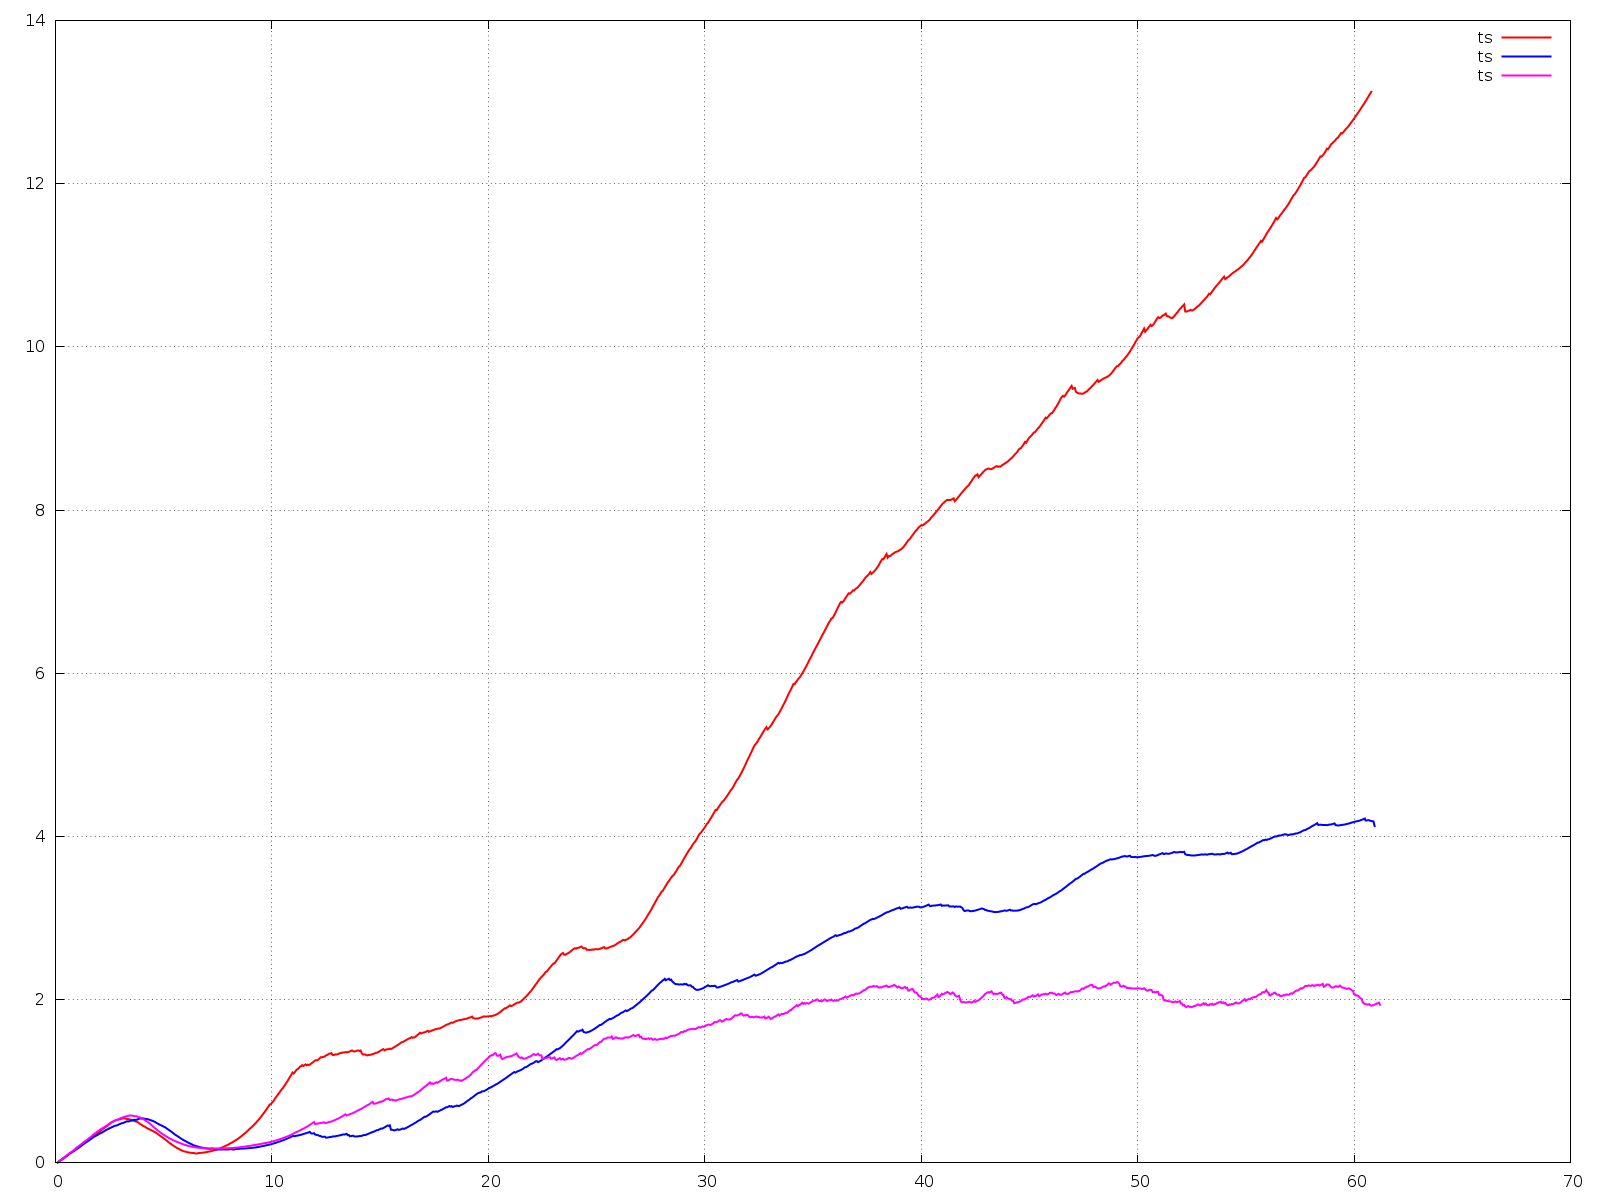
\includegraphics[width=\linewidth]{all_50_ts.png}
    \caption{3 алгоритма, 50 юнитов, "устаревание" секторов от времени}
\end{figure}

\clearpage
\newpage
